% Created 2020-12-27 Sun 23:59
% Intended LaTeX compiler: pdflatex
\documentclass[sigconf,natbib,screen=true,review=true,anonymous]{acmart}

% We'll get the submission number fro the submission system
\acmSubmissionID{2043}

% !TEX root = ./main.tex

% list your packages
\usepackage[utf8]{inputenc}
\usepackage[T1]{fontenc}
\usepackage{graphicx}
\usepackage{grffile}
\usepackage{longtable}
\usepackage{wrapfig}
\usepackage{rotating}
\usepackage[normalem]{ulem}
%\usepackage{amsmath}
\usepackage{textcomp}
%\usepackage{amssymb}
\usepackage{capt-of}
\usepackage{hyperref}
%\usepackage{minted}

\usepackage{algorithmic}
\usepackage{graphicx}
\usepackage{xcolor}
\usepackage{multirow} 
\usepackage{xcolor}
\usepackage[ruled,linesnumbered,boxed]{algorithm2e}
\usepackage[inline]{enumitem}
\usepackage{booktabs}
\usepackage[skip=0pt]{caption}
\usepackage{acronym}
\usepackage{url}
% \usepackage{graphicx}
% \usepackage{adjustbox}

\usepackage{xcolor}

%\usepackage{amsmath}
\usepackage{dsfont}
\usepackage{color}

% !TEX root = ./main.tex

% list your definitions
\newcommand{\mdr}[1]{\textcolor{orange}{\textbf{[#1]}}}
\newcommand{\daan}[1]{\textcolor{teal}{\textbf{[DO: #1]}}}
\newcommand{\mvm}[1]{\textcolor{blue}{\textbf{[MvM: #1]}}}
\newcommand{\hvk}[1]{\textcolor{pink}{\textbf{[HVK: #1]}}}

\newcommand\todo[1]{\textcolor{red}{TODO : #1}}
\newcommand\doubt[1]{\textcolor{orange}{DOUBT : #1}}
% \newcommand\todo[1]{} % uncomment to hide comments
% \newcommand\doubt[1]{} % uncomment to hide comments

\hypersetup{
 pdfauthor={Gabriel Bénédict},
 pdftitle={},
 pdfkeywords={},
 pdfsubject={},
 pdfcreator={Emacs 26.1 (Org mode 9.1.14)},
 pdflang={English}}

% !TEX root = ./main.tex

\author{Gabriel B\'en\'edict}
\affiliation{
\institution{RTL \& University of Amsterdam} 
\city{Amsterdam}
\country{The Netherlands}
}
\email{something}

\author{Daan Odijk}
\affiliation{
\institution{RTL} 
\city{Amsterdam}
\country{The Netherlands}
}
\email{something}

\author{Maarten de Rijke}
\affiliation{
\instutute{University of Amsterdam \& Ahold Delhaize}
\city{Amsterdam}
\country{The Netherlands}
}
\email{m.derijke@uva.nl}

% !TEX root =  ./main.tex 

\copyrightyear{2021}
\acmYear{2021}
\setcopyright{rightsretained}
\acmConference[SIGIR '21]{Proceedings of the 44th International ACM SIGIR Conference on Research and Development in Information Retrieval}{July 11-15, 2021}{Montr{\'{e}}al, Canada}
\acmBooktitle{Proceedings of the 44th International ACM SIGIR Conference on Research and Development in Information Retrieval (SIGIR '21), July 11-15, 2021, Montr{\'{e}}al, Canada}
\acmPrice{}
\settopmatter{printfolios=false}

\begin{CCSXML}
<ccs2012>
   <concept>
       <concept_id>10002951.10003317.10003347.10003356</concept_id>
       <concept_desc>Information systems~Clustering and classification</concept_desc>
       <concept_significance>500</concept_significance>
       </concept>
   <concept>
       <concept_id>10002951.10003317.10003318.10003321</concept_id>
       <concept_desc>Information systems~Content analysis and feature selection</concept_desc>
       <concept_significance>300</concept_significance>
       </concept>
 </ccs2012>
\end{CCSXML}

\ccsdesc[500]{Information systems~Clustering and classification}
\ccsdesc[300]{Information systems~Content analysis and feature selection}

\keywords{Content analysis; Classification; Multilabel classification; Custom loss functions}


\begin{document}


\title[sigmoidF1: A Smooth F1 Score Surrogate Loss for Multilabel Classification]{sigmoidF1: A Smooth F1 Score Surrogate Loss for Multilabel Classification}
  % SIMPUL: A Loss Framework to Learn Abstract Labels from Abstract Representations: Single-Instance Multiclass Multilabel Prediction with Unknown Label Count}

\begin{abstract}

  Multiclass multilabel classification refers to the task of attributing multiple labels to examples via predictions. Current models formulate a reduction of that multilabel setting into either multiple binary classifications or multiclass classification, allowing for the use of existing loss functions (sigmoid, cross-entropy, logistic, etc.). Empirically, these methods have been reported to achieve good performance on different metrics (F1 score, Recall, Precision, etc.). Theoretically though, the multiclass classification reduction does not allow one to predict varying numbers of labels per example, because the underlying losses are distant estimates of the performance metrics.\daan{This suggests a theoretical contribution.}

  We propose a loss function, sigmoidF1. It is an approximation of the F1 score that (I) is smooth and tractable for stochastic gradient descent, (II) naturally approximates a multilabel metric, (III) estimates label propensities and label counts. More generally, we show that any confusion matrix metric can be formulated with a smooth surrogate. We evaluate the proposed loss function on different text and image datasets, and with a variety of metrics, to account for the complexity of multilabel classification evaluation. In our experiments, we embed the sigmoidF1 loss in a classification head that is attached to state-of-the-art efficient pretrained neural networks MobileNetV2 and DistilBERT.

Our experiments show that sigmoidF1 outperforms other loss functions on four datasets and several metrics. These results show the effectiveness of using inference-time metrics as loss function at training time in general and their potential on non-trivial classification problems like multilabel classification.

\if0
its smooth -> section 3.1 & figure 1
naturally approximate the multilabel metric of choice -> experimental results, table 3

(label count and label prediction)

maybe remove the correlation claim YES

add that we give the first formalization of unboundedF1

instead of reformulating the estimand entirely, we just allow it to be stochastic instead of deterministic.

by definition reg(f_n)


people usually implement this methods with cross-entropy, we flollow in their footsteps.

leave multiclass classification

\fi


% \mdr{Multilabel classification is the task of classifying XXX.}
% \mdr{In multilabel classification with unknown label counts we do not know XXX.}
% \mdr{Multilabel classification with unknown label counts are very common in IR.}
% \mdr{Current approaches to Multilabel classification with unknown label counts are characterized by XXX and suffer from YYY.}
% \mdr{We propose XXX to address Multilabel classification with unknown label counts.}
% \mdr{We evaluate our proposal on XXX.}
% \mdr{We find XXX.}
% \mdr{Broader implications.}
\if0
Multilabel classification is a common task when learning from text, image, or sound. However, few optimization frameworks are tailored towards learning multiple abstract labels for an entire text, image, or sound. State of the art models for image and text, of the CNN and BERT family respectively, are often benchmarked on multiclass multilabel datasets, but still use loss functions adapted to a multiclass unilabel situation (i.e. variations of cross-entropy losses).

When the number of ground-truth labels varies over each example as is commonly the case in multilabel classification, these losses produce unit-interval results that require a sophisticated thresholding regime (at training or at inference time) to predict both label prediction propensity and label count.

Since certain confusion matrix metrics usually already fulfill that goal at inference time, we propose decomposable surrogates for gradient descent at training time. We illustrate the solution with \emph{sigmoidF1}: a decomposable surrogate F1 score that introduces smooth thresholding. We are able to demonstrate its performance on efficient versions of the state of the art models (DistilBert and MobileNetV2). For a fair assessment of the proposed loss function, we avoid datasets that would benefit from a two stage modeling procedure (object / expression / segment detection followed by classification) and instead turn to datasets, where the whole example is predictive of a label.
\fi
\end{abstract}


\maketitle

\acresetall

\setlength{\belowdisplayskip}{0.5\baselineskip} \setlength{\belowdisplayshortskip}{0.5\baselineskip}
\setlength{\abovedisplayskip}{0.5\baselineskip} \setlength{\abovedisplayshortskip}{0.5\baselineskip}

% !TEX root = ../main.tex

\section{introduction}
\label{sec:org662677c}

As neural network models are able to learn increasingly more abstract representations via deeper networks, representation learning and self-supervision~\citep[see, e.g.,][]{XX,YYY,ZZZ}, it is reasonable to expect that they also get better at predicting more abstract labels. 
Beyond identifying object types~\mdr{REF}, performing face recognition~\mdr{REF}, \mdr{doing what with} expressions~\mdr{REF}, neural networks should soon be able to predict genres/categories of text, image and sound at high levels of accuracy. 
Towards this goal, there is a significant volume of recent work on building neural networks with high-level of understanding in the embedding space~\mdr{REF}.
However, there seems to be limited research on developing loss functions that are adapted for these higher level concepts in the output space.

\mdr{Briefly and concretely describe the abstract labeling task that we are interested in.}

To situate the specific problem that we tackle in this paper, it is helpful to consider Figure~\ref{fig:tree} so as to disambiguate our terminology. 
Figure~\ref{fig:tree} shows \mdr{what}.
There seems to exist a consensus over the terms \emph{multiclass} and \emph{multilabel learning}, meaning mutually exclusive and mutually inclusive labels, respectively \todo{source}. 
Multilabel learning can therefore be seen as a subdomain of multiclass learning, where more than one class can be true for the same example. 
Within multilabel training, we introduce the distinction between multi-instance multilabel~\citep[e.g.,][]{multiInstance}) and uni-instance multilabel. 
\mdr{vague: Multi-instance multilabel classification refers to tasks where elements within each example can be singled-out and assigned one or more labels; examples include objects \mdr{not a task} in an image or tokens in a text.}
Uni-stance multilabel classification is \mdr{define it}.
\begin{itemize}
\item \mdr{Now explain that the task introduced in the second paragraph is an instance of uni-instance multilabel classification.}
\item \mdr{Now make the distinction between fixed label counts and varying label counts}
\item \mdr{Little work has been done on the uni-instance, ML MC prediction with a varying number of classes}
\item \mdr{Identify the shortcomings o prior work on the task that we care about}
\end{itemize}

\begin{figure}[t]
\centering
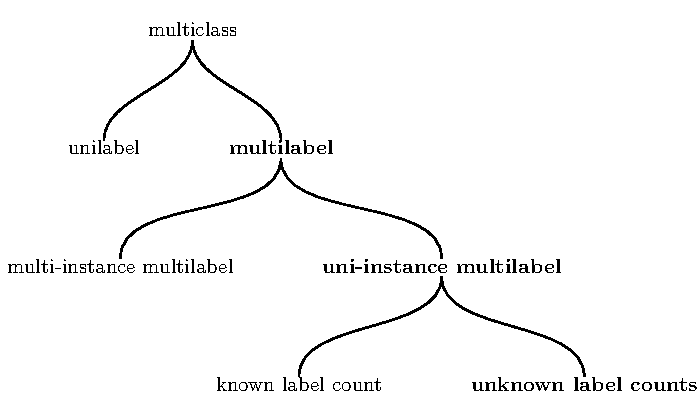
\includegraphics[width=.9\linewidth]{./tree/Tree.pdf}
\caption{\label{fig:tree}
Clarifying ``multiclass'' classification problems.}
\end{figure}

\mdr{Now we have a paragraph in which you clearly describe your proposed line of attack}

\mdr{Now we have a paragraph that explains the results that we have obtained with our proposed approach}

\mdr{Now we have a paragraph with our main contributions:}
\begin{itemize}[leftmargin=*]
\item \mdr{Contribution 1}
\item \mdr{Contribution 2}
\item \mdr{Contribution 3}
\end{itemize}

\mdr{The remainder of the paper is organized as follows. Expand.}

\vspace*{3cm}
\mdr{Move all of the content to other sections, e.g., to background section or to related work. Also, try to avoid the meandering narrative that touches on many points but sometimes forgets to make explicit what its main point is.}

In this paper we focus on uni-instance multilabel training (sparse occurences of the term holistic can be found in the literature to describe this phenomenon for image \cite{holisticImageDescriptors,holisticLungs} and a recent video dataset \cite{holisticVideoData} \todo{read these}), more specifically with varying label counts. To the best of our knowledge, there are few existing representatives of that type of labelling task in the literature. \todo{cite more milestone examples for each category.} \todo{delta with hierarchical label learning}

\mdr{Too talkative, too many diverse angles. Make sure that there is a clear point that you are making:}
Although multilabel binary prediction (commonly referring to mutually inclusive labels) is a task thoroughly covered in existing literature, there does not seem to exist a framework that deals with different amounts of positive labels in the groundtruth. For example, a scientific journal can be tagged as \emph{machine learning} and \emph{economics}, or a movie can be tagged as \emph{romance} and \emph{comedy}. These instances might as well be assigned only one tag in the groundtruth, or many more within the possible tags (classes).


The particularity of tasks like scientific paper tagging or movie genre classification is that it remains unclear what elements in an image/video or text can be singled out as predictive of a particular tag/genre. Rather, a complex interaction between these elements in the feature space steer the predictions. For example, the sole mention of the term "machine learning" in a paper should not be a sufficient condition to tag it as such. Instead, one could expect from the publisher to get acquainted with the paper enough to determine wether the research is a worthwhile contribution or application of \emph{machine learning} to deserve the tag. This involves thorough understanding of the proposed method and background knowledge on state-of-the-art methods. An analogous argument can be made for movie genre classification for movie posters.

However, if elements in an image/text can be singled out as predictive of a single tag, the problem reverts back to predicting with the a priori knowledge of the existence of only one true label (i.e. multi-instance multilabel learning).  The reason for distanciating singling-out from uni-instance labels, is that it has been shown that as soon as singling-out is possible, models that work on instances are more accurate \todo{rewrite this paragraph and sources}. The singled-out elements can be subsets of the original feature space (typically in object detection like with the COCO dataset  \cite{COCO} or the Amazon Rainforest Dataset\footnote{Available at \url{https://www.kaggle.com/c/planet-understanding-the-amazon-from-space}} \todo{others}). Similarly, recent research has shown that the singled-out elements can be located in the abstract representations (embeddings) of the feature set and might individually predict a single true label (like GPT-3 \todo{source}) \todo{more examples}. This might also carry prospects of generalizability of the model \cite{generalization} \todo{elaborate}. 

But for now, in certain retrieval tasks such as scientific journal tagging, the effect of sub-entities (either expressions in the text or single features in the embedding space) on the prediction of each label remains hard to assess. Instead we propose uni-instance (sometimes referred to as holistic) multilabel learning for varying amount of labels, with a focus on custom loss functions.

To allow the use of existing diffentiable loss fonctions, previous research papers tend to reframe the problem into either (I) a multi-instance multiclass (as described above, with the COCO dataset as an example of isolation of features \cite{COCO}), (II) uni-instance multiclass prediction (III) uni-instance multilabel prediction with fixed label count (IV) uni-instance multilabel prediction with varying label count with post-training thresholding (V) redefine backpropagation for multilabel prediction \cite{multilabelBackprop} (VI) multitask learning \cite{multitaskLabel} (VII) custom loss function \cite{tencent}. This order reflects in ascending order how close modelling seem to fit the original task, which remains uni-instance multilabel learning with varying amounts of labels. \doubt{group them}

Common loss functions such as cross-entropy loss (for mutually inclusive labels) or multinomial logit loss (for mutually exclusive labels) deliver predictions on the unit interval. Thresholding the output to assess the performance of the model against the groundtruth can be done after training for (I), (II), (III) and (IV). \todo{give a very sound reason as to why we'd rather not do things post-training and rather at training-time}. Problem formulations (V), (VI) and (VII) suggest a solution at training time. We think that a custom loss function (VII) is the best alternative. \todo{explain why}

In a number of retrieval tasks, a model's out of sample accuracy is measured on metrics such as AUROC, F1 score, etc. These reflect an objective catered towards evaluating the model over an entire ranking. Due to to lack of differentiability, these metrics cannot be directly used as loss functions at training time (in-sample). A seminal study \cite{optimizableLosses} derived a general framework for deriving decomposable surrogates to some of these metrics. We propose our own decomposable F1 surrogate tailored for the problem at hand.

\mdr{This paragraph can probably be kept in the introduction}
We first propose a general mathematical formulation of uni-instance multilabel learning for varying amount of groundtruth labels. The generalization encompasses different levels of complexity, from the classical cross-entropy loss up to the proposed loss function. \emph{sigmoidF1} is a F1 score surrogate which allows to optimize for label prediction and count simultanuously in a single task and is robust to outliers. It delivers more precise predictions than the current state-of-the-art on several different metrics, accross text and image related tasks. \emph{sigmoidF1} and its adaptive \emph{SadF1} and Bayesian \emph{SBayesF1} counterparts are benchmarked against loss functions commonly used in multilabel learning and others tailored specifically to the uni-instance multilabel with varying number of labels setting.

% !TEX root = ../main.tex

\section{Background, Learning algorithms for FIMPUL problems}
\label{section:background}

\todo{put this paragraph somewhere, it is a justification for FIMPUL}
 Beyond identifying object types (see YOLO~\cite{YOLO} and its successors), performing face recognition (see FaceNet\cite{FaceNet} and its successors) on segments of an image, neural networks
are increasingly becoming better at predicting more abstact concepts via
deeper networks, representation learning and self-supervision~\citep[see,
e.g.,][]{SS,Rep}. Towards this goal, there is a significant volume of recent
work on building neural networks with a high-level of abstract understanding
in the embedding space~\mdr{REF}. However, research on developing optimization
frameworks that are adapted for these abstract concepts in the output space is
limited.

This section introduces the terminology and our mathematical formulation of solutions to multilabel classification with unknown label count on full instances.

% \textbf{we introduce our sub-problem}

The FIMPUL problem definition of \textbf{F}ull-\textbf{I}nstance\textsuperscript{(3)} \textbf{M}ultilabel\textsuperscript{(2)} \textbf{P}rediction for \textbf{U}nknown\textsuperscript{(4)} \textbf{L}abel counts is shortly disambiguated here. There seems to exist a consensus over the terms \emph{multiclass learning} and
\emph{multilabel learning}. They denote settings of mutually exclusive and non-mutually exclusive labels \footnote{non-mutually exclusive means here one example can have more than one label}, respectively~\cite{multilabelMethods}. Multilabel learning can
therefore be seen as a subdomain of multiclass learning, where more than one
class can be correct for the same example. We propose the term full-instance
as opposed to multi-instance learning~\citep[e.g.,][]{multiInstance,
multiInstanceMultiLabel}, for which it is considered natural to first segment
an image, text or sound before performing prediction on each of the segments. Most importantly, we propose loss functions suited for situations where the label count for each document / image is unknown.

% \textbf{current state of the art, related work}
The existing optimization frameworks are still largely based on variations of
the cross-entropy loss, with recently some advances in dealing with
sparsity in the output space~\citep[see, e.g.,][]{focalLoss,tencent}. Existing measures for multilabel prediction can be
divided into two fields: the \emph{fit-data-to-algorithm} (a.k.a \emph{problem tranformation}) and \emph{fit-algorithm-to-data} (a.k.a \emph{algorithm adaptation}) approaches~\cite{multilabelReview}. Although it is less in use in the literature, we prefer the former definitions because they are less ambiguous. In the case of fit-data-to-algorithm,
multilabel classification is reframed as a binary, multiclass classification
or label ranking problem. In the case of fit-algorithm-to-data, one tries to
adapt multiclass algorithms to the problem.

\subsection{fit-data-to-algorithm} We define a learning algorithm that maps inputs to outputs given a set of hyperparameters \(\mathcal{F}(\cdot ; \Theta): \mathcal{X} \rightarrow \mathcal{Y}\). For the purpose of fit-data-to-algorithm,
we define \(\mathcal{L}_{\text {multiclass}}\), a class of loss functions that
minimize predictions in relative terms. Binary cross-entropy, logistic regression and their
variants, such as focal loss or hinge loss are common choices when it comes to
multiclass prediction. Cross-entropy loss can be formulated as
\(\mathcal{L}_{\text {CE}}=-\sum \log \left(p_{i}\right)\). Note that
minimizing binary cross-entropy is equivalent to maximizing for log-likelihood
\cite[Section 4.3.4]{Bishop}. More generally, the fit-data-to-algorithm formulation amounts to minimizing the loss on a class of neural networks, such that
%
\begin{equation}
\underset{\mathcal{L}_{\text {multiclass}}} {\min} \mathcal{F}\left(\cdot ;
\Theta; \mathcal{L}_{\text {multiclass}} (\mathbf{y}, \hat{\mathbf{y}})
\right),
\end{equation}
%

This class of loss functions is particularly useful for multiclass unilabel predictions or multiclass multilabel predictions with known amount of labels $k_i$ per example/document $i$. In the former case,  we can select top-1 label predictions and in the latter top-k. Note that one common approach in fit-data-to-algorithm is to establish a hierarchical structure in labels. This way, one can constrain the algorithm to learn only 1 or $k$ labels per group in the hierarchy. For example, DBPedia\footnote{https://wiki.dbpedia.org/develop/datasets/latest-core-dataset-releases} establishes a hierarchical structure in wikipedia infoboxes\footnote{https://en.wikipedia.org/wiki/Help:Infobox} and is commonly used to finetune state-of-the-art NLP models~\citep[see, e.g.,][]{XLNet, ULMFit}.

There are however datasets for which reducing the problem to top-k selection and/or establishing a hierarchical structure would be an oversimplification. Certain datasets have classes that are not mutually exclusive, whether or not they are ordered in a hierarchy (aside from the movie and paper datasets chosen for experiments, we briefly mention music datasets in the related work section). 

\subsection{fit-algorithm-to-data}
In the context of fit-algorithm-to-data, a combination of existing algorithms are used to deal with non-mutually exclusive classes. The aim is to
both obtain a propensity of each label being true and a prediction of the
number of true labels:
%
\begin{equation}
\underset{\mathcal{L}_{\text {multiclass}}, \mathcal{L}_{\text {count}}}
{\min} \mathcal{F}\left(\cdot ; \Theta; \mathcal{L}_{\text {multiclass}}
(\mathbf{y}, \hat{\mathbf{y}}) + \lambda \mathcal{L}_{\text {count}}
(\mathbf{n}, \hat{\mathbf{n}})\right),
\end{equation}
%
where \(n_i = \sum_j \mathds{1}_{\mathbf{y_i^j} = 1}\) is the count of
positive labels per example. We thus impose a constraint for the retrieval of
label counts. For example, a cross-entropy loss surrogate would penalize for the number of wrongly predicted
labels \(\mathcal{L}_{\text {CE+N}}= \mathcal{L}_{\text {CE}} + \lambda (\sum
tp / \sum p)\), with \(t p=\sum_{i \in Y^{+}} \mathds{1}_{\mathbf{p_i} \geq
b}\) and \(b\) a threshold to be defined. The fit-algorithm-to-data
formulation is most straightfoward but suffers from higher parametrization and
the lack of modelling of the interactions between label counts and label
prediction.


\subsection{Current Limitations}

In summary, in the case of \emph{fit-data-to-algorithm},
cross-entropy losses are used at training time and thresholding is done at
inference time. In the case of \emph{fit-algorithm-to-data}, elements of the
learning algorithm are changed (such as the backpropagation procedure or the
tasks).

In machine learning prediction tasks, the probabilistic measure (or a reversible
transformation of a probabilistic measure such as a sigmoid or a softmax
function) are compared to binary values in the case of binary encoding of
classes. At training time, if the number $n_i$ of labels to be predicted per
example is known a priori, it is natural to assign the $top_{n_i}$ predictions
to that example~\cite{lossTopKError, topKmulticlassSVM}. If the number of
labels per example is unknown a priori, the question remains at training and at inference time
as to how to extract information about the number of labels to assign to each
example, aside from the propensity of labels to be assigned. This is generally
done via a \emph{decision threshold}, that can be set globally for all
examples. This threshold can optimize for specificity or
sensitivity~\cite{decisionThreshold}. We propose a method where this threshold
is implicitely defined, thanks to the use of metrics that already penalize for
wrong label counts.

\todo{reference fig}
See figure \ref{fig:knee}.


\begin{figure}[htbp]
\centering
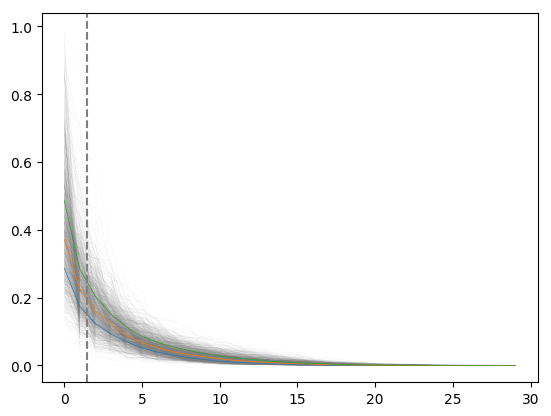
\includegraphics[width=.9\linewidth]{./images/knee.png}
\caption{\label{fig:knee}
\todo{nicer plot on another dataset (this is from RTL)}
Ordered per-label cross-entropy predictions for each example (each grey line) with the median (orange) and IQR (green \& blue) over all examples. Determining a global threshold can be related to visually finding the ``knee'' in that median curve (dotted line).}
\end{figure}


\subsection{design-algorithm-for-data}

With design-algorithm-for-data, we suggest to design loss functions to address FIMPUL problems specifically. We first formulate a unified loss, namely
%
\begin{equation}
\underset{\mathcal{L}_{\text {multilabel}}} {\min} \mathcal{F}\left(\cdot ;
\Theta; \mathcal{L}_{\text {multilabel}} (\mathbf{y}, \hat{\mathbf{y}},
\mathbf{n}, \hat{\mathbf{n}}) \right),
\end{equation}
%
Although predictions and counts explicitly appear in that formulation,
\(\mathcal{L}_{\text {multilabel}}\) can optimize for both metrics implicitly
(see proposed \emph{sigmoidF1} below). This way, the correlation between label count and label predictions is embedded in the loss. Furthermore, we avoid having to mitigate the importance of label prediction VS label count with a regularizer  $\lambda$. For that purpose, we use surrogates of classical statistical and Information Retrieval metrics.

In a number of retrieval tasks, a model's out of sample accuracy is measured
on metrics such as AUROC, F1 score, etc. These reflect an objective catered
towards evaluating the model over an entire ranking. Due to the lack of
differentiability, these metrics cannot be directly used as loss functions at
training time (in-sample). A seminal study~\cite{optimizableLosses} derived a
general framework for deriving decomposable surrogates to some of these
metrics. We propose our own decomposable surrogates tailored for the problem
at hand.

The proposed design-algorithm-for-data method is thus an alternative to fit-data-to-algorithm and fit-algorithm-to-data. design-algorithm-for-data uses metric as losses, allows for dynamic thresholding and implicitly deals with label counts and label predictions.

% \begin{figure}[t]
% \centering
% 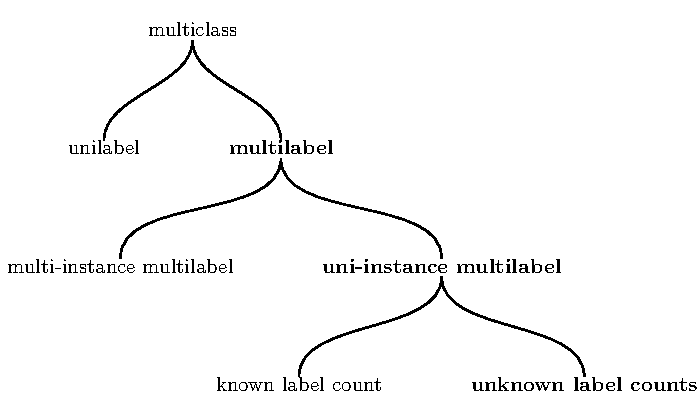
\includegraphics[width=.9\linewidth]{./tree/Tree.pdf}
% \caption{\label{fig:tree} SIMPUL (bold) within the \emph{multiclass}
% nomenclature
% \hvk{figure is not referenced in text, bold is unclear in figure}
% \daan{I think it should go. And if it stays: uni -> single.}
% % Clarifying ``multiclass'' classification problems. In this paper we focus on
% % the uni-instance, multilabel, multiclass classification problem with a
% % varying number of labels (the bottom right hand side of the tree).
% }
% \end{figure}% \mdr{Image source ...}

%%% Local Variables:
%%% mode: latex
%%% TeX-master: "../main"
%%% End:

% !TEX root = ../main.tex

\section{Method}
\label{sec:orga8a42f5}
\label{section:method}

In this section, we introduce our approach for multilabel problems, with a Confusion Matrix Metric as a loss. In evaluation of multilabel or multiclass problems, confusion matrix metrics are a common choice, because they implicitly deal with label count. In our framework, we leverage a smoothed version of the confusion matrix that can be used to directly optimize as a loss function (the original confusion matrix metrics rely on step functions and are therefore intractable). Before we discuss smoothing the confusion matrix metrics, we first briefly recap our learning setting and define the confusion matrix metrics in this setting more formally.

\begin{figure}[tbp]
\centering
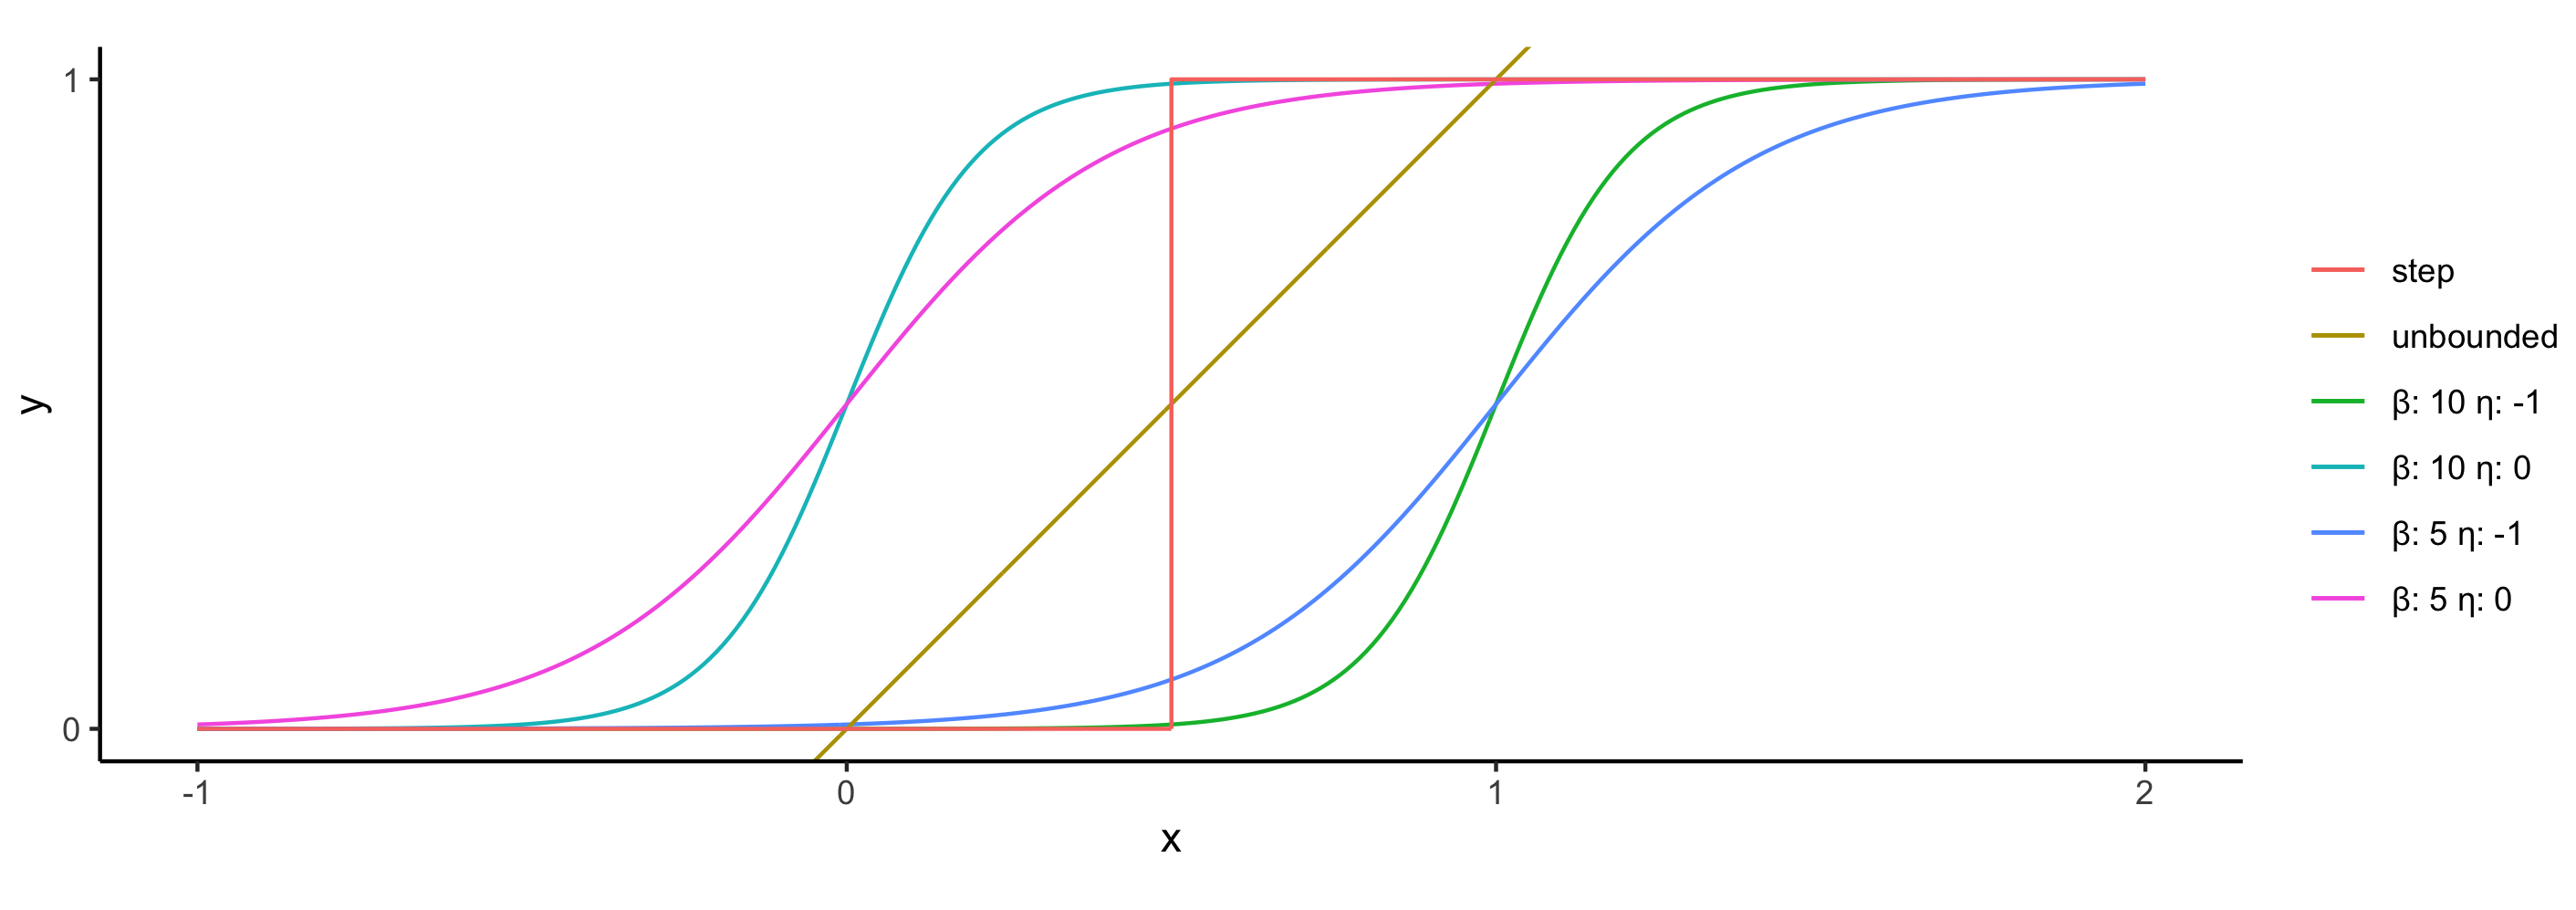
\includegraphics[width=\linewidth]{./images/sigmoid.png}
\caption{\label{fig:sigmoid}
Different thresholding regimes: the non-decomposable step function, the unbounded linear function and the sigmoid function at different parametrizations}\todo{Redraw for single column.}
\end{figure}
\label{fig:sigmoid}

% For the same class of learning algorithms defined in the previous section \(\mathcal{F}(\cdot ; \Theta): \mathcal{X} \rightarrow \mathcal{Y}\), we consider a particular case, where \(\mathbf{x} = \{x_1, \ldots, x_n\}\) and each observation is assigned $k$ labels (one or more) \(\mathbf{l} = \{l_1, \ldots, l_C\}\) out of a set of classes $C$. \(y_{i}^{j}\) are binary variables, indicating presence of a label for each observation \(i\) and class \(j\).

% For each observation \(i\), label class probabilities can be defined based on predictions as

% \todo{check this formula}

% \begin{equation}
% \mathbf{p}_{i}=\left\{\begin{array}{ll}\hat{\mathbf{y}} & \text { if } y=1 \\ 1-\hat{\mathbf{y}} & \text { otherwise }\end{array}\right.
% \end{equation}

We use the binary classification setting (two classes) as it simplifies the notation and prevents further use of subscripts or matrix operations, without loss of generalization to the multiclass case.
In a typical binary classification problem with the label vector $\mathbf{y} = \{y_1 , \ldots, y_n\}$, predictions are probabilistic and it is necessary to define a threshold \(t\), at which a prediction is dichotomized. With \(\mathds{1}\) as an indicator function, \(Y^+ = \sum \mathds{1}_{\hat{\mathbf{y}} \geq t}\), \(Y^- = \sum \mathds{1}_{\hat{\mathbf{y}} < t}\) are thus the count of positive and negative predictions at threshold \(t\). Let \(tp\), \(fp\), \(fn\), \(tn\) be number of true positives, false positives, false negatives and true negatives respectively:
%
\begin{equation}
\label{eq:conf}
\begin{array}{ll}\mathit{tp} = \sum \mathds{1}_{\hat{\mathbf{y}} \geq t} \odot \mathbf{y}  & \mathit{fp} = \sum \mathds{1}_{\hat{\mathbf{y}} \geq t} \odot (\mathds{1} - \mathbf{y}) \\[.5em] \mathit{fn} = \sum \mathds{1}_{\hat{\mathbf{y}} < t} \odot \mathbf{y} & \mathit{tn} = \sum \mathds{1}_{\hat{\mathbf{y}} < t} \odot (\mathds{1} - \mathbf{y}),
\end{array}
\end{equation}
%
%, \(\sum^+\) and \(\sum^-\) corresponding to  \(\sum_{i \in Y^{+}}\) and \(\sum_{i \in Y^{-}}\) respectively
with \(\odot\) the component-wise multiplication sign.


For simplicity, in the formulation above and the ones that follow scores are calculated for a single class, therefore the sum is implicitly over all examples \(\sum_i\). This is useful for the binary classification problem but also for the multilabel problem, when micro metrics are calculated (i.e. metric for each class which is then averaged over all classes, see end of this section, where we further refine the micro and macro concepts). In the multilabel setting $\mathbf{y}$ can be substituted by $\mathbf{y}^j$ for each class $j$. Note that vectors could be trivially substituted by matrices ($Y$) in the following expressions to obtain the macro formulation.


% In the multilabel setting $\mathbf{y}$ can be substituted by $\mathbf{y}^j$ for each class $j$. Note that vectors could be trivially substituted by matrices ($Y$) in the following expressions to obtain the macro formulation.
% \doubt{do you agree that the subscript for the sum is implicit? and do you agree that the matrix formulation is trivial?}\hvk{do we really need this paragraph?}
% \daan{I think we should drop this.}

% Note that Equation \ref{eq:conf} represents a macro measure. For example, the micro $tp$ measure (i.e. for each class) would be $\sum \mathds{1}_{\hat{\mathbf{y}} \geq b} \odot \mathbf{y}$ $\sum_{i \in \hat{\mathbf{y}}^{j+}} \mathds{1}_{\hat{y}^{j}_{i} \geq b} \odot y^{j}_{i}$ (see end of this section, where we further refine the micro and macro concepts).

Given the four confusion matrix quadrants, we can generate further metrics like precision and recall (see Table \ref{tab:confusion-matrix}). However none of these metrics are decomposable due to the hard thresholding which is in effect a step function (see Figure \ref{fig:sigmoid}).

In the following sections, we first define desirable properties for decomposable thresholding.
Next, we define unbounded confusion matrix entries and a notion of sigmoid-based transformation that renders confusion matrix entries decomposable. Finally, we focus on an unbounded F1 score wich we use in our experiments.

\subsection{Desirable properties of decomposable thresholding}
\label{subsection:properties}

We thus define desirable properties for a decomposable sign function $f(u)$ as a surrogate of the above indicator function \(\mathds{1}_{\hat{\mathbf{y}} < t}\).

\begin{property}
  Boundedness: $|f(u)| < M$, where $M$ is an upper and lower bound.
\end{property}
The groundtruth $\mathbf{y}$ is bounded between $[0,1]$ and thus it must be compared to a bounded prediction $\mathbf{\hat{y}}$, preferably bounded by $[0,1]$, to avoid further scaling.

\begin{property}
  Saturation: $\int_{s}^{\infty} f^{-1}(u) = \int_{-\infty}^{-s} f(u) = \epsilon$, with $\epsilon$ a number close to zero and $s$ a saturation bound.
\end{property}
For the surrogate to be a proper sign function substitute, it is important to often return values close to 1 or 0. Saturation is defined in the context of neural network activation functions and refers to the propensity of iterative backpropagation to progressively lead to values very close to 0 or 1 after a long enough training period. While activation functions should tend to be non-saturated, in order for the derivative at point $u$ to be non-null and information to flow back to the network~\cite{saturation}, our sign function substitute must output values close to 0 or 1, in order to be comparable to a step function.

\begin{property}
  Dynamic Gradient: $f'(u) \gg 0 \quad \forall \; u \in [-s, s]$, where $s$ is the saturation bound.
\end{property}

Inside the saturation bounds $[-s, s]$, the derivative should be significantly higher than zero in order to facilitate stochastic gradient descent and backpropagation.

Note that the upper and lower limits of $f(u)$ are interchangeably $[-1,1]$ or $[0,1]$ along this paper and in the literature. The conditions above still apply by linear transformation.

In the following we show how our formalization of an unbounded F1 surrogate would not fulfill these properties and how our proposition of smooth bounded alternative does.


\subsection{Unbounded confusion matrix entries}
\label{subsec:unbounded}

A first trivial remedy to allow for derivation of the sign function, is to define \emph{unbounded} confusion matrix entries by replacing the dichotomized predictions with prediction probabilities. This way,
 (i.e. \(\overline{tp}\), \(\overline{fp}\), \(\overline{fn}\) and  \(\overline{tn}\) are not natural numbers anymore):
%
\begin{equation}
\label{eq:unbounded}
\begin{array}{ll} \overline{\mathit{tp}} = \sum \hat{\mathbf{y}} \odot \mathbf{y}  & \overline{\mathit{fp}} = \sum \hat{\mathbf{y}} \odot (\mathds{1} - \mathbf{y}) \\[.5em] \overline{\mathit{fn}} = \sum (\mathds{1} - \hat{\mathbf{y}}) \odot \mathbf{y} & \overline{\mathit{tn}} = \sum (\mathds{1} - \hat{\mathbf{y}}) \odot (\mathds{1} - \mathbf{y}),
\end{array}
\end{equation}
%
% $$
% \overline{tp}=\sum \hat{\mathbf{y}} \odot \mathbf{y} \quad \overline{fp} = \sum \hat{\mathbf{y}} \odot (\mathbf{1}- \mathbf{y}) \quad \overline{fn} = \sum (\mathbf{1} - \hat{\mathbf{y}}) \odot \mathbf{y}
% $$

\(tp\), \(fp\), \(fn\) and \(tn\) are now replaced by rough surrogates. The disadvantages are that the desirable properties mentioned above are not fulfilled, namely (i) \(\hat{\mathbf{y}}\) is unbounded and thus certain examples can have over-proportional effects on the loss, (ii) It is non-saturated. While non-saturation is desirable for activation functions~\cite{saturation}, it would be here desirable to tend towards saturation (i.e. tend to values close to 0 or 1, so as to give the most accurate predictions at any thresholding values at inference time). (iii) The gradient of that linear function is 1 and therefore backpropagation will not learn depending on different inputs at this stage of the loss function.

However, this method has the advantage of resulting in a linear loss function that avoids the concept of thresholding altogether and is trivial to decompose for stochastic gradient descent.

\subsection{Smooth confusion matrix entries}

We propose a sigmoid-based transformation of the confusion matrix that renders its entries decomposable and fulfills the three properties above:
%
\begin{equation}
\label{eq:smooth}
\begin{array}{ll} \widetilde{\mathit{tp}} = \sum \mathbf{S}(\hat{\mathbf{y}}) \odot \mathbf{y}  & \widetilde{\mathit{fp}} = \sum \mathbf{S}(\hat{\mathbf{y}}) \odot (\mathds{1} - \mathbf{y}) \\[.5em] \widetilde{\mathit{fn}} = \sum (\mathds{1} - \mathbf{S}(\hat{\mathbf{y}})) \odot \mathbf{y} & \widetilde{\mathit{tn}} = \sum (\mathds{1} - \mathbf{S}(\hat{\mathbf{y}})) \odot (\mathds{1} - \mathbf{y}),
\end{array}
\end{equation}
%
with $\mathbf{S}(\cdot)$ the vectorial form of the sigmoid function $S(\cdot)$:
%
\begin{equation}
S(u; \beta, \eta)=\frac{1}{1+\exp (-\beta (u + \eta))},
\end{equation}
%
with \(\beta\) and \(\eta\) tunable parameters for slope and offset respectively. Higher \(\beta\) results in steeper slope at the center of the sigmoid and thus more stringent thresholding. At its extreme, \(\lim_{\beta\to\infty} S(u; \beta, \eta)\) corresponds to the step function used in Equation \ref{eq:conf}. Note that negative values of $\beta$ geometrically reflect the sigmoid function across the horizontal line at $0.5$ and thus invert predictions.


These smooth confusion matrix entries allow to build any related metric (see Table \ref{tab:confusion-matrix}). Furthermore, the surrogate entries are decomposable, bounded, saturated and have a dynamic gradient.

\begin{table*}[]
\caption{Confusion matrix with our proposed smoothed confusion matrix entries, $\widetilde{\mathit{tp}}$, $\widetilde{\mathit{fp}}$, $\widetilde{\mathit{fn}}$ and $\widetilde{\mathit{tn}}$ and six derived loss functions that use these smoothed confusion matrix entries. $\mathcal{L}_{\widetilde{\mathit{F1}}}$ is used in our experiments.}
\label{tab:confusion-matrix}
\def\arraystretch{1.1}
\begin{tabular}{|c||c|c||c|} \cline{2-4}
\multicolumn{1}{l|}{} & \textbf{Condition} & \textbf{Condition} & \multirow{2}{*}{$\mathcal{L}_{\widetilde{\mathit{Accuracy}}}= \frac{\widetilde{\mathit{tp}} + \widetilde{\mathit{tn}}}{\widetilde{\mathit{tp}} + \widetilde{\mathit{fp}} + \widetilde{\mathit{tn}} + \widetilde{\mathit{fn}}}$} \\
\multicolumn{1}{l|}{} & \textbf{positive} &  \textbf{negative} & \\ \hline \hline
\textbf{~Predicted~} & True positive & False positive & \multirow{2}{*}{$\mathcal{L}_{\widetilde{\mathit{Precision}}}= \frac{\widetilde{\mathit{tp}}}{\widetilde{\mathit{tp}} + \widetilde{\mathit{fp}}}$} \\
\textbf{positive} & $\widetilde{\mathit{tp}}=\sum \mathbf{S}(\hat{\mathbf{y}}) \odot \mathbf{y}$ & $\widetilde{\mathit{fp}}= \sum \mathbf{S}(\hat{\mathbf{y}}) \odot (\mathds{1} - \mathbf{y})$ & \\ \hline
\textbf{Predicted} & False negative & True Negative & \multirow{2}{*}{$\mathcal{L}_{\widetilde{\mathit{NPV}}}= \frac{\widetilde{\mathit{tn}}}{\widetilde{\mathit{tn}} + \widetilde{\mathit{fn}}}$} \\
\textbf{negative} & $\widetilde{\mathit{fn}}= \sum (\mathds{1} - \mathbf{S}(\hat{\mathbf{y}})) \odot \mathbf{y}$ & $\widetilde{\mathit{tn}}= \sum (\mathds{1} - \mathbf{S}(\hat{\mathbf{y}})) \odot (\mathds{1} - \mathbf{y})$ & \\ \hline \hline
\multicolumn{1}{l|}{} & \multirow{2}{*}{\hspace{1.2em}$\mathcal{L}_{\widetilde{\mathit{Recall}}}= \frac{\widetilde{\mathit{tp}}}{\widetilde{\mathit{tp}} + \widetilde{\mathit{fn}}}$\hspace{1.2em}}& \multirow{2}{*}{$\mathcal{L}_{\widetilde{\mathit{Specificity}}}= \frac{\widetilde{\mathit{tn}}}{\widetilde{\mathit{fp}} + \widetilde{\mathit{tn}}}$} & \multirow{2}{*}{$\mathcal{L}_{\widetilde{\mathit{F1}}}= \frac{\widetilde{\mathit{tp}}}{2 \widetilde{\mathit{tp}}+ \widetilde{\mathit{fn}}+ \widetilde{\mathit{fp}}}$} \\
\multicolumn{1}{l|}{} & & & \\
\cline{2-4}
\end{tabular}%
\end{table*}

In this paper we focus on sigmoidF1 ($\mathcal{L}_{\widetilde{\mathit{F1}}}$) because it has the ability to implicitly penalize for both inacurate label propensity and label count.


\subsection{Smooth macro F1 scores}
\label{sec:orgc5d29d7}

While smoothness is defined above, there is yet a precision to make about micro-averaging versus macro-averaging in multilabel-classification problems. Micro-averaging is biased by class frequency, whereas macro-averaging regards all classes as equally important. \emph{unboundedF1} and \emph{sigmoidF1} below are thought of as macro scores (aggregated over all classes). These scores require a high enough number of representatives in the four confusion matrix quadrants to learn from batch to batch. Ideally, each training epoch would have only one batch, so as to have the most representatives.

Following Equation \ref{eq:unbounded}, it is possible to define an \emph{unbounded F1} score. A formulation similar to \emph{unboundedF1} was proposed in an unpublished blog post, which was referred to as \emph{softF1}~\cite{softF1}. We define our \emph{unbounded F1} score as follows:
%
\begin{equation}
\mathcal{L}_{\overline{\mathit{F1}}}= \frac{\overline{tp}}{2 \overline{tp}+ \overline{fn}+ \overline{fp}}
\end{equation}
%
While this alternative abstracts the thresholding away, which is convenient for fine-tuning purposes, it does not fulfil the desirable properties of a dichotomization threshold surrogate. For more on that see Section~\ref{subsec:unbounded}.

\emph{unboundedF1} will be used to benchmark against our proposed \emph{sigmoidF1} loss. Given the definitions of smooth confusion matrix metrics above, we can now write $\mathcal{L}_{\widetilde{\mathit{F1}}}$.
%
\begin{equation}\label{eq:sigmoidF1}
\mathcal{L}_{\widetilde{\mathit{F1}}}= \frac{\widetilde{\mathit{tp}}}{2 \widetilde{\mathit{tp}}+ \widetilde{\mathit{fn}}+ \widetilde{\mathit{fp}}}
\end{equation}
%
A similar method was proposed outside of the context of neural networks: the \emph{Maximum F1-score criterion} for automatic mispronunciation detection as an objective function to a Gaussian Mixture Model-hidden Markov model (GMM-HMM)\cite{sigmoid}.

\emph{sigmoidF1} is particularly suited for the multilabel setting because it is a proper hard thresholding surrogate as defined in the previous sections and because it contains a significant amount of information about label prediction accuracy: $\widetilde{\mathit{tp}}$, $\widetilde{\mathit{fn}}$ and $\widetilde{\mathit{fp}}$ are indicative of the number of predicted labels in each category of the confusion matrix but also contain a notion of certainty, given that they are rational numbers. The built in sigmoid function ensures that certainty increases along training epochs, as outlined by proposition 2. Finally, as the harmonic mean of precision and recall (A property of F1 in general), it weighs in both relevance metrics.

\vspace{\baselineskip}

We end this section by writing down the focal loss~\cite{focalLoss}, as it deals specifically with class imbalance and is used as a baseline due to its popularity in the multiclass domain.
%
\begin{equation}
  \mathcal{L}_{FL} = -\alpha^{\mathrm{j}}\left(1-\hat{y}^{\mathrm{j}}\right)^{\gamma} \log \left(\hat{y}^{\mathrm{j}}\right),
\end{equation}
%
with $\alpha^j$ and $\gamma$ hyperparameters. In the next section, we further specify the setup for focal loss and cross entropy as benchmarks for \emph{unboundedF1} and \emph{sigmoidF1}.

% Given the presence of the step indicator function \(\sum \mathds{1}_{\mathbf{p_i} \geq b}\), \(F_\beta\) is not differentiable for gradient based methods. One way of surpassing that problem is to use a surrogate.

% \subsection{soft F1 score}
% \label{sec:org3ca83ef}

 % with smooth confusion matrix entries :



% /softF1/ is
% $$\mathcal{L}_{\text {Pred}}=\sum_{i, j}\left(\mathbf{y}_{i j}-\hat{\mathbf{y}}_{i j}\right)^{2}$$

% \subsection{sigmoidF1 score}
% \label{sec:orgc5d29d7}


% \begin{figure}[htbp]
% \centering
% 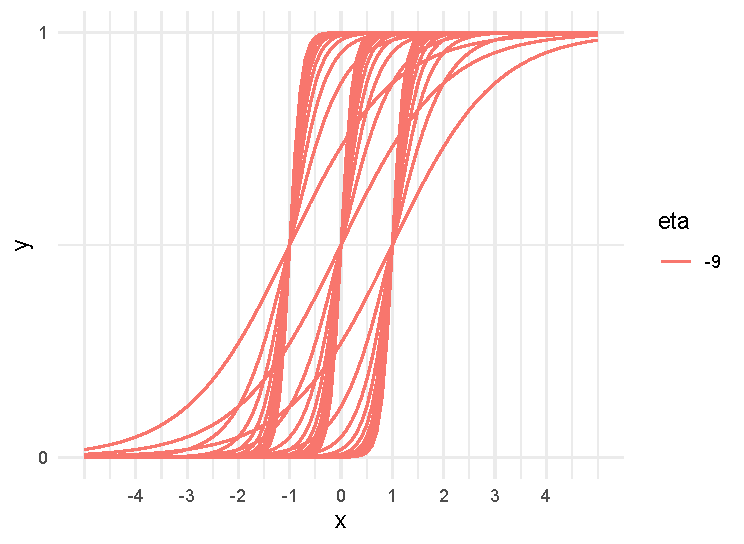
\includegraphics[width=.9\linewidth]{./images/sigmoid.pdf}
% \caption{\label{fig:sigmoid}
% Sigmoid function with different values for $\beta$ (steepness) \& $\eta$ (offset)}
% \end{figure}

%  with \(S(u)\), the confusion matrix entries then become

% \begin{equation}\label{eq:sigmoidF1}
% \widetilde{\mathit{tp}}=\sum S(\hat{\mathbf{y}}) \odot \mathbf{y} \quad\widetilde{\mathit{fp}}= \sum S(\hat{\mathbf{y}}) \odot (\mathbf{1} - \mathbf{y}) \quad \widetilde{\mathit{fn}}= \sum (\mathbf{1} - S(\hat{\mathbf{y}})) \odot \mathbf{y}
% \end{equation}

% And thus

% \begin{equation}
% \mathcal{L}_{\text {sigmoidF1}}= \frac{\widetilde{\mathit{tp}}}{2 \widetilde{\mathit{tp}}+ \widetilde{\mathit{fn}}+ \widetilde{\mathit{fp}}}
% \end{equation}

% \doubt{mention smooth hinge loss} \cite{smoothHinge}

% $\doublewidetilde{tp}$
% https://tex.stackexchange.com/questions/321231/double-widetilde
% doesn't work


% \todo{explain batch size mathematically for F1 surrogate losses}


%%% Local Variables:
%%% mode: latex
%%% TeX-master: "../main"
%%% End:

% !TEX root = ../main.tex

\section{Experimental Setup}
\label{sec:orgb44ba25}

We test multilabel learning using our proposed sigmoidF1 loss function on four datasets across different modalities, consisting of image and text. 
The datasets each fit the FIMPUL characteristics. In particular, they are best modeled with full-instance learning as the entire image or the full text is predictive of the instance's labels. The next section and Table~\ref{table:datasets} describe our four datasets. The learning architecture, in which a classification head attached to a pretrained net, is then described before addressing hyperparameter tuning and reproducibility remarks.

\begin{table}[b]
\caption{Descriptive statistics of our experimental datasets.}
\label{table:datasets}
\centering
% \begin{adjustbox}{max width=\textwidth}
\begin{tabular}{l rrrr}
\toprule
& & & Average & Number of \\
& Type & Classes & label count & examples \\
\midrule
moviePosters & image & 28 & 2.165 & 37,632\\
arXiv2020 & text & 155 & 1.888 & 26,558\\ 
chemExposure & text & 38 & 6.116 & 3,661\\
cancerHallmarks\hspace{-.7em}  & text & 33 & 3.501 & 1,582\\
\bottomrule
\end{tabular}
% \end{adjustbox}
\end{table}

\subsection{Datasets}

Our first dataset comes from the vision domain and consists of movie posters and their genres (e.g., \emph{action}, \emph{comedy}).\footnote{Labels available at \url{https://tinyurl.com/y7ydyedu} and prescraped images from IMDB at \url{https://tinyurl.com/y7lfpvlx}.} The posters and labels have been extracted from IMDB and the dataset was previously used for per-class, post-training thresholding \citep{moviePosters} (see Section~\ref{sec:org2aceb9f}). The genre labels in this dataset are not mutually exclusive and of varying counts per movie. 

We use the newly created \emph{arXiv dataset}\footnote{Available at \url{https://www.kaggle.com/Cornell-University/arxiv}} with over 1.7 million open source articles and their metadata. Our experiments use the abstracts and categories that are suitably non-mutually exclusive and of varying counts per example. There is a longer history of using arXiv to create research datasets; the dataset we use is not to be confused with an earlier long document dataset that only features 11 classes~\citep{oldarXiv}, but was used in a recent long transformer publication~\cite{bigBird}. The limited number of labeled classes render the older dataset unsuitable for our experiments.  We write \textit{arXiv2020} for the subset of the \emph{arXiv dataset} that only contains documents published in 2020, given limited computing power. This results in around 26k documents.

\begin{figure*}[!tp]
\centering
     \begin{subfigure}{0.6\linewidth}
         \centering
         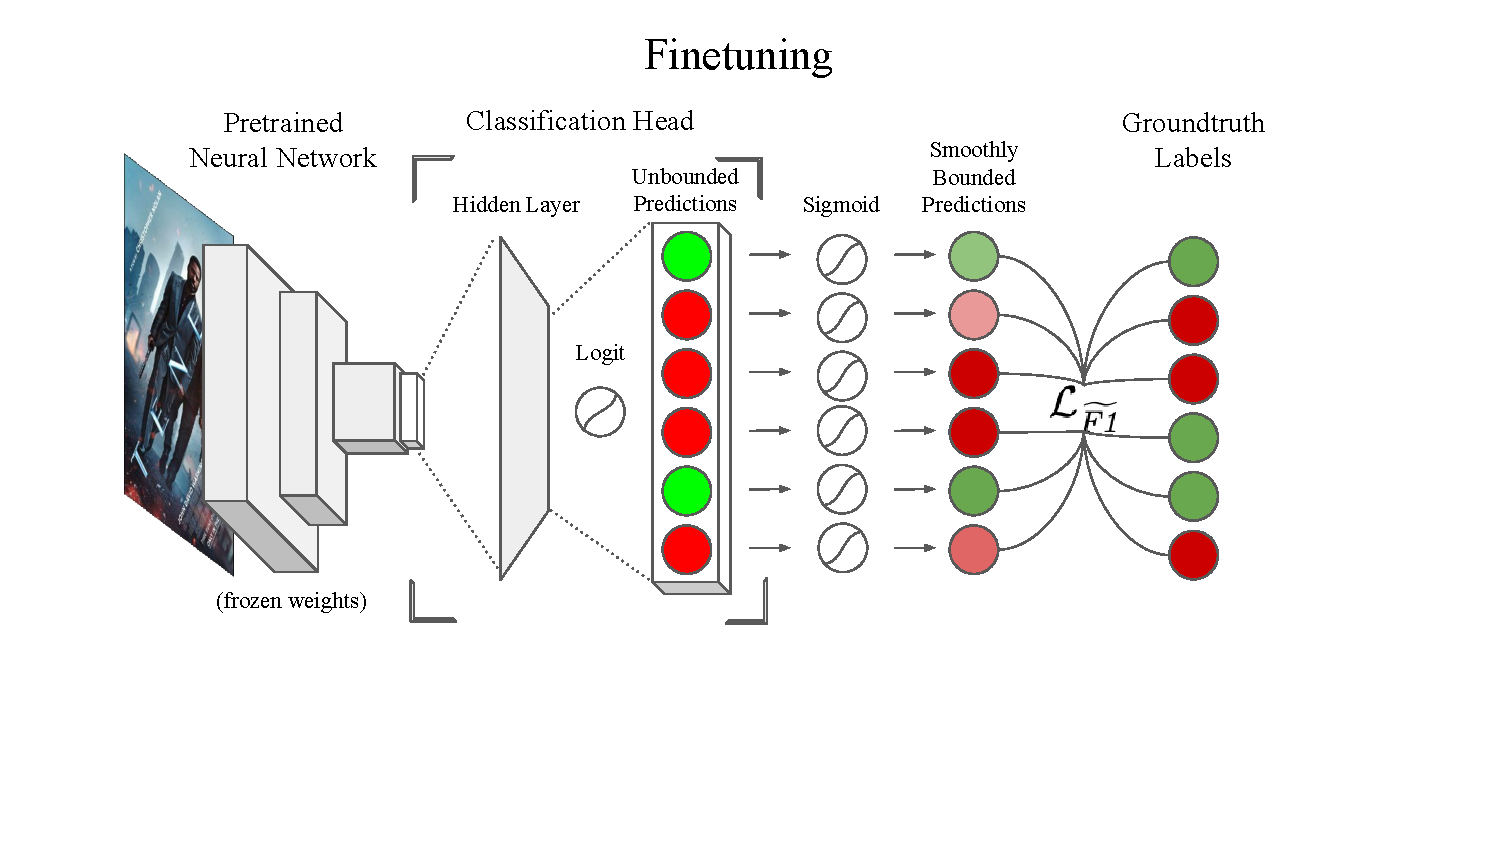
\includegraphics[page=1,width=\linewidth,trim=80 100 110 0,clip]{images/SIGIR2021 Loss Diagram.pdf}
         \caption{Finetuning of a pretrained neural network with an adapted classification head and using sigmoidF1 as a loss function..}
     \end{subfigure}
     \hspace{.02\linewidth}
     \begin{subfigure}{0.36\linewidth}
         \centering
         \includegraphics[page=2,width=\linewidth,trim=190 100 210 0,clip]{images/SIGIR2021 Loss Diagram.pdf}
         \caption{During inference, unbounded predictions are transformed to predictions with a Softmax.}
     \end{subfigure}
     \vspace{.5\baselineskip}
\caption{Learning framework used in the CoMMaL framework and specifically for sigmoidF1 as a loss function.}
\label{fig:architecture}
\end{figure*}

To the best of our knowledge, ML-NET~\cite{multitaskLabel} is the state-of-the-art among \emph{fit-algorithm-to-data} methods for multilabel learning with unknown label count on text (the work does not differentiate full-instance and multi-instance learning, see Section~\ref{sec:org2aceb9f}). Among the three datasets used for benchmarking ML-NET, the cancerHallmark~\citep{cancerHallmarks}\footnote{Available at \url{https://github.com/sb895/Hallmarks-of-Cancer}} and chemicalExposure~\citep{chemExposure}\footnote{Available at \url{https://github.com/sb895/chemical-exposure-information-corpus}} datasets are of multi-instance multilabel nature: several expressions are annotated within each paper abstracts. The third dataset diagnosisCodes could not be obtained (neither from the authors of ML-NET nor of the original paper~\cite{diagnosisCode}). We treat cancerHallmarks and chemicalExposure as full-instance datasets by aggregating expression labels over each example, as was done for ML-NET.

\subsection{Learning framework}

The learning framework consists of two parts: a pretrained deep neural network and a classification head (see Figure \ref{fig:architecture}); the classification head is where we slot in alternative loss functions.

Since the focus of this paper is in comparing loss functions and not neural network architectures, we chose efficient network architectures in terms of accuracy and computation.
For the moviePoster image dataset, we use a MobileNetV2~\cite{mobileNet} architecture that was pretrained on ImageNet~\cite{imagenet}. This network architecture is typically used for inference on small computing devices (e.g., smartphones). We use a version of MobileNetV2 already stripped off of its original classification head.\footnote{The pretrained network can be loaded here \url{https://tfhub.dev/google/imagenet/mobilenet_v2_100_224/feature_vector/4}.}
For the three text datasets, we use DistilBert~\cite{distilBert} as implemented in Hugging Face. This is a particularly efficient instance of the BERT model.\footnote{The pretrained network can be loaded here \url{https://huggingface.co/transformers/model_doc/distilbert.html}.}.
In both cases, we use the final pretrained layer as an embedding of the input. In order to make sure that the results of different loss functions are comparable, we fix the model weights of the pretrained MobileNetV2 and DistilBert and keep the hyperparameter values that were used to train them from scratch. We also initialize the model weights with the same TensorFlow internal random seeds across training sessions.

A similar classification head is used for both MobileNetV2 and DistilBert. It consists of a latent representation layer (the final pretrained layer mentioned above) connected with a RELU activation. This layer is linked to a final classification layer with a linear activation. The dimension of the final layer is equal to the number of classes in the dataset. When computing focalLoss and crossEntropy, a softmax transformation transforms the unbounded last layer to a $[0,1]$ bounded vector. When computing sigmoidF1 loss, a sigmoid transformation is operated instead, which results in a sparser $[0,1]$ vector. At inference time, the last layer is used for prediction and is bounded with a softmax function. A threshold must then be chosen at evaluation time to compute different metrics. Figure \ref{fig:architecture} depicts this learning framework. Thresholding regimes at inference time are further discussed in Sections~\ref{sec:evalMetrics} and~\ref{subsec:thresh}.

% \gab{ev. remove losses compared}
% \subsection{Losses Compared}
% \label{section:losssescompared}

% We benchmark sigmoidF1 against three other losses. The cross-entropy loss and its variant for sparse datasets, focal loss, are representatives of the fit-data-to-algorithm approach as they are binary classifiers. The third loss function is unboundedF1 and represents a first step towards CoMMaL.
 
\subsection{Evaluation metrics}
\label{sec:evalMetrics}

In our experimental evaluation, we consider a suite of metrics that are commonly used in the evaluation of multilabel classification to measure the effectiveness of multilabel prediction. Such metrics are based on the confusion matrix that we detailed in Section~\ref{section:method} and for which we provided smoothed surrogates to optimize directly.

When true positives and false positives are used, recall that \(t p=\sum_{i \in Y^{+}} \mathds{1}_{\mathbf{p_i} \geq t}\) and \(f p=\sum_{i \in Y^{-}} \mathds{1}_{\mathbf{p_i} \geq t}\), and thus a threshold \(t\) must be set. Information on thresholding at inference time is generally hard to find in the recent literature, we thus decide on neutral thresholds before training. For arXiv2020 and moviePosters, we set \(t = 0.5\), as is commonly done in the early literature~\cite{multilabelReview, ML-DT}.
For the two medical datasets, cancerHallmarks and chemicalExposure, we saw after a few preparatory training rounds that only sigmoidF1 had non-zero results for \(t = 0.5\). Information is a lot more sparse for these dataset, we thus set the evaluation metrics threshold to a reasonable value of $0.05$ and train for $500$ epochs until reaching convergence. 

Extending \(F_1\) to multi-class binary classification amounts to deciding wether or not to pool classes.
In a first pooled iteration, macro \(F_1\)~\cite{multilabelMetrics} equates to creating a single 2x2 confusion matrix for all classes:
%
\begin{equation}
F_1^{macro} = \frac{\sum^c tp_j}{2 \sum^c tp_j + \sum^c fn_j + \sum^c fp_j},
\end{equation}
%
with $\sum^c (\cdot)$ as a short form of $\sum_{j=1}^c(\cdot)$, when summing over each class up to the $c$'th class.
Micro \(F_1\) \cite{threshForF1, multilabelMetrics} amounts to creating one confusion matrix per class or unpooling:
%
\begin{equation}
F_1^{micro} =  \frac{1}{c} \sum_{j=1}^c \frac{tp_j}{2 tp_j + fn_j + fp_j} =  \frac{1}{c} \sum_{j=1}^c F_1^j.
\end{equation}
%
Weighted micro \(F_1\)~\cite{weightedMetrics} is similar but includes weighing to account for class imbalance, i.e., weighing each class by the number of ground-truth positives:
%
\begin{equation}
F_1^{weighted} = \frac{1}{c} \sum_{j=1}^c p_j F_1^j \quad \text{, where } p_j = \sum_i \mathds{1}_{\mathbf{y_i^j} = 1}.
\end{equation}
%
We also define micro precision% and micro recall
%
\begin{equation}
\begin{aligned} P^{micro} &=  \frac{1}{c} \sum_{j=1}^c \frac{tp_j}{tp_j+fp_j}% \\ R^{micro} &=  \frac{1}{c} \sum_{j=1}^c \frac{tp_j}{tp_j+fn_j}
\end{aligned}
\end{equation}
%
In our experiments, we report on weightedF1, microF1, macroF1, Precision% and Recall
. Macro scores do not differentiate multiclass unilabel classification from multiclass multilabel classification. Micro scores treat classes separately. The \emph{weighted} micro F1 score is a further refinement where class scores are weighted by their representation in the dataset. We thus focus our discussion of experimental results around weightedF1 as we consider this to be the most representative for success on FIMPUL problems. 

There is an interaction between our optimization on sigmoidF1 and our evaluation using (weighted) F1 metrics. If our approach of optimizing for an F1 surrogate succeeds, we expect higher values on F1-related metrics during evaluation. For this reason, we consider and discuss not a single, but multiple metrics.

\subsection{Hyperparameters and reproducibility}
\label{subsec:hypers}

We choose to ignore classes that are underrepresented, in order to give the model a fair chance at learning from at least a few examples. We define underrepresentation as a global irrelevance threshold $b$ for classes: any class $c$ that is represented less than $b$ times is considered irrelevant. We decided to set an irrelevance threshold $b$ on all datasets prior to conducting experiments, so as to not finetune for that feature. It was set to 1000 for both \emph{arXiv2020} (145 of the original 155 classes remaining) and \emph{moviePosters} (14 of the 28 classes remaining) and at 10 for \emph{chemicalExposure} (all 38 classes remaining) and \emph{cancerHallmarks} (all 33 classes remaining), in proportion to the number of classes and labels in each dataset.

Batch size is set at a high value of 256. We thus increase accuracy over traditional losses~\cite{bigBSArxiv}, but also allow heterogeneity in the examples within the batch, thus collecting enough values in each quadrant of the confusion matrix (see Section \ref{sec:orgc5d29d7} for a discussion on batch sizes).

Regarding the sigmoidF1 hyperparameters $\beta$ and $\eta$, we performed a grid search with the values in the range $[1,30]$ for $\beta$ and $[0, 2]$ for $\eta$.
In our experiments, we evaluate the sensitivity of our method to these hyperparameters (see Figure~\ref{fig:sigmoid}).

We made sure to split the data in the same training, validation and test sets for each loss function. Our code, dataset splits and other settings are shared to ensure reproducibility of our results. 

We performed our experiments on Amazon Web Services cloud machines with parallelization on up to 16 GPUs \textit{p2.16xlarge}, with TensorFlow 2 as a gradient-descent backend.

% !TEX root = ../main.tex

\section{Experimental Results}
\label{sec:orgc23a664}





We show results on four different datasets, moviePosters, cancerHallmarks, chemicalExposure and Arxiv2020.

In general, we observe that sigmoidF1 performs better on most metrics and across different datasets. macroSoftF1 however systematically outperforms all other measures on Precision. 

FocalLoss, which is specifically tailored for sparse data, does not perform well here. Note that macroSoftF1 can be particularly performent without requiring hyperparameter tuning. Across Tables \ref{tab:chemicalExposure, tab:moviePosters, tab:arxiv2020, tab:cancerHallmarks} we see that the smooth sigmoidF1 outperforms other existing losses. Although only the metrics@0.5 are shown, where 0.5 is the dichotomization threshold, the ablation study and our open sourced code further illustrates the consistent good performance of sigmoidF1 versus other losses.


For the two medical datasets cancerHallmarks and chemicalExposure, information is a lot more sparse, we thus set the evaluation metrics threshold at 0.05 and train for 500 epochs until reaching convergence. 

\todo{change to percentage}

\begin{table}[htbp]
  \caption{Movie posters (CNN). \mdr{Explain what we see.}}
  \label{tab:moviePosters}
\centering
\begin{tabular}{l ccccc}
\toprule 
Loss  & \rotatebox{90}{macroF1 @ 0.5} & \rotatebox{90}{microF1 @ 0.5} & \rotatebox{90}{weightedF1 @ 0.5} & \rotatebox{90}{Precision @ 0.5} & \rotatebox{90}{Recall @ 0.5}\\ 
\midrule
$\mathcal{L}_{\text {CE}}$ & 0.051 & 0.186 & 0.149 & 0.090 & 0.042 \\ 
$\mathcal{L}_{\text {FL}}$ & 0.055 & 0.192 & 0.154 & 0.115 & – \\
% $\mathcal{L}_{\text {CE+N}}$ & 0 & 0 & 0 & 0 & 0 \\
$\mathcal{L}_{\text {macroSoftF1}}$ & 0.136 & 0.207 & 0.243 & \textbf{0.105} & 0.190 \\
$\mathcal{L}_{\text {sigmoidF1}}$ & \textbf{0.158} & \textbf{0.224} & \textbf{0.300} & 0.104 & \textbf{0.557} \\ % run aa424792a57e4208ad1805cd6e63f8e6
\bottomrule
\end{tabular}
\end{table}


\begin{table}[htbp]
  \caption{Arxiv (distillBERT 2020), frozen pretrained weights 100 epochs, min-label-thresh: 1000}
  \label{tab:arxiv2020}  
\centering
\begin{tabular}{l ccccc}
\toprule
Loss  & \rotatebox{90}{macroF1 @ 0.5} & \rotatebox{90}{microF1 @ 0.5} & \rotatebox{90}{weightedF1 @ 0.5} & \rotatebox{90}{Precision @ 0.5} & \rotatebox{90}{Recall @ 0.5}\\ 
\midrule
$\mathcal{L}_{\text {CE}}$ & 0.093 & 0.106 & 0.106 & 0.096 & – \\ % Run 71ef078f975649d5b3d897e504bc638b
$\mathcal{L}_{\text {FL}}$ & 0.008 & 0.011 & 0.009 & 0.054 & 0.954 \\
% $\mathcal{L}_{\text {CE+N}}$ & 0 & 0 & 0 & 0 & 0 \\
$\mathcal{L}_{\text {macroSoftF1}}$ & 0.077 & 0.088 & 0.087 & \textbf{0.100} & – \\ % run 405a6e6851e84a89a82313251a7a36e8 (18-19 jan)
$\mathcal{L}_{\text {sigmoidF1}}$ & \textbf{0.093} & \textbf{0.106} & \textbf{0.106} & 0.096 & \textbf{–} \\ % run bd478ca55eb64cc78d9ad0f25accce35 (18-19 jan)
\bottomrule
\end{tabular}
\end{table}

\begin{table}[htbp]
  \caption{Cancer Hallmarks}
  \label{tab:cancerHallmarks}
\centering
\begin{tabular}{l ccccc}
\toprule 
Loss  & \rotatebox{90}{macroF1 @ 0.05} & \rotatebox{90}{microF1 @ 0.05} & \rotatebox{90}{weightedF1 @ 0.05} & \rotatebox{90}{Precision @ 0.05} & \rotatebox{90}{Recall @ 0.05}\\ 
\midrule
$\mathcal{L}_{\text {CE}}$ & 0.0 & 0.0 & 0.0 & 0.0 & 0.0 \\ 
$\mathcal{L}_{\text {FL}}$ & 0.044 & 0.190 & 0.108 & 0.071 & 0.055 \\
% $\mathcal{L}_{\text {CE+N}}$ & 0 & 0 & 0 & 0 & 0 \\
$\mathcal{L}_{\text {macroSoftF1}}$ & \textbf{0.098} & 0.176 & 0.170 & \textbf{0.089} & 0.131 \\
$\mathcal{L}_{\text {sigmoidF1}}$ & 0.095 & \textbf{0.313} & \textbf{0.202} & 0.059 & \textbf{0.264} \\ % run e145056949424b02bfc83cc57af38374
\bottomrule
\end{tabular}
\end{table}


\begin{table}[htbp]
  \caption{Chemical Exposure}
  \label{tab:chemicalExposure}
\centering
\begin{tabular}{l ccccc}
\toprule
Loss  & \rotatebox{90}{macroF1 @ 0.05} & \rotatebox{90}{microF1 @ 0.05} & \rotatebox{90}{weightedF1 @ 0.05} & \rotatebox{90}{Precision @ 0.05} & \rotatebox{90}{Recall @ 0.05}\\ 
\midrule
$\mathcal{L}_{\text {CE}}$ & 0.012 & 0.058 & 0.051 & 0.047 & 0.007 \\ % Run 71ef078f975649d5b3d897e504bc638b
$\mathcal{L}_{\text {FL}}$ & 0.0934 & 0.348 & 0.268 & 0.130 & 0.091 \\
$\mathcal{L}_{\text {macroSoftF1}}$ & \textbf{0.133} & 0.194 & 0.218 & \textbf{0.155} & 0.138 \\ % run 405a6e6851e84a89a82313251a7a36e8 (18-19 jan)
$\mathcal{L}_{\text {sigmoidF1}}$ & 0.113 & \textbf{0.432} & \textbf{0.319} & 0.091 & \textbf{0.188} \\ % run a30825efe9c94a24bc46a9c71a5f8646 E: 0.5 S: 0.6
\bottomrule
\end{tabular}
\end{table}


\subsection{Sensitivity Analysis}

\begin{figure}[htbp]
\centering
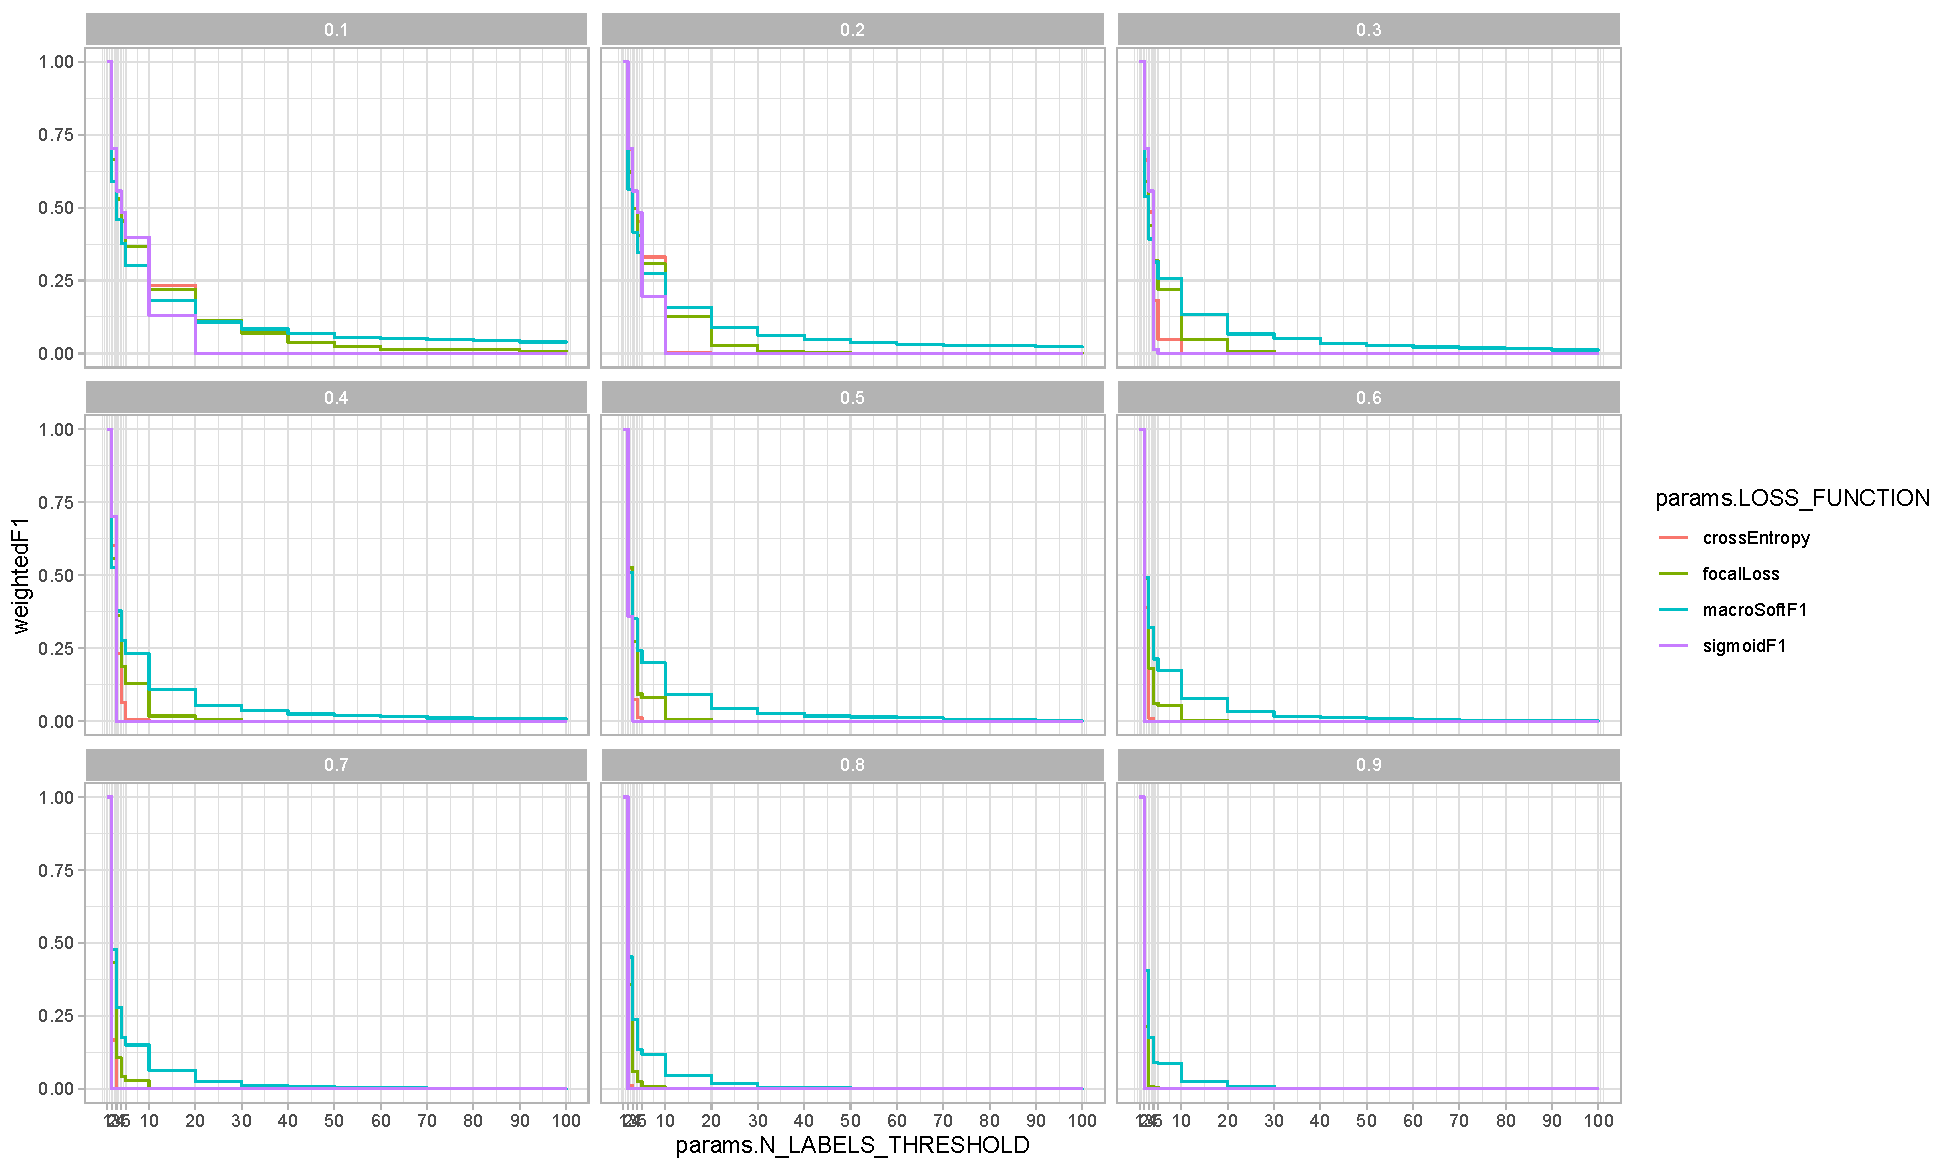
\includegraphics[width=.9\linewidth]{./images/ablation.pdf}
\caption{\label{fig:etaBeta}
weighted F1 score at different threshold (x axis) and for different values of Eta and Beta. Dots connected with a line are from the same experiment.}
\end{figure}




\subsection{Ablation Study - Arxiv2020}

We performed an analysis of sensitivity to different amount of labels. For this, the irrelevance threshold (see definition in Section \ref{sec:orgb44ba25}) $t$ was set to the values 0, 10, 100 and 1000. This time, results are shown with dichotomization thresholds of 0.1 to 0.9. \todo{see if keep it}

\todo{sensitivity to hyperparametertuning plot}

\begin{figure}[htbp]
\centering
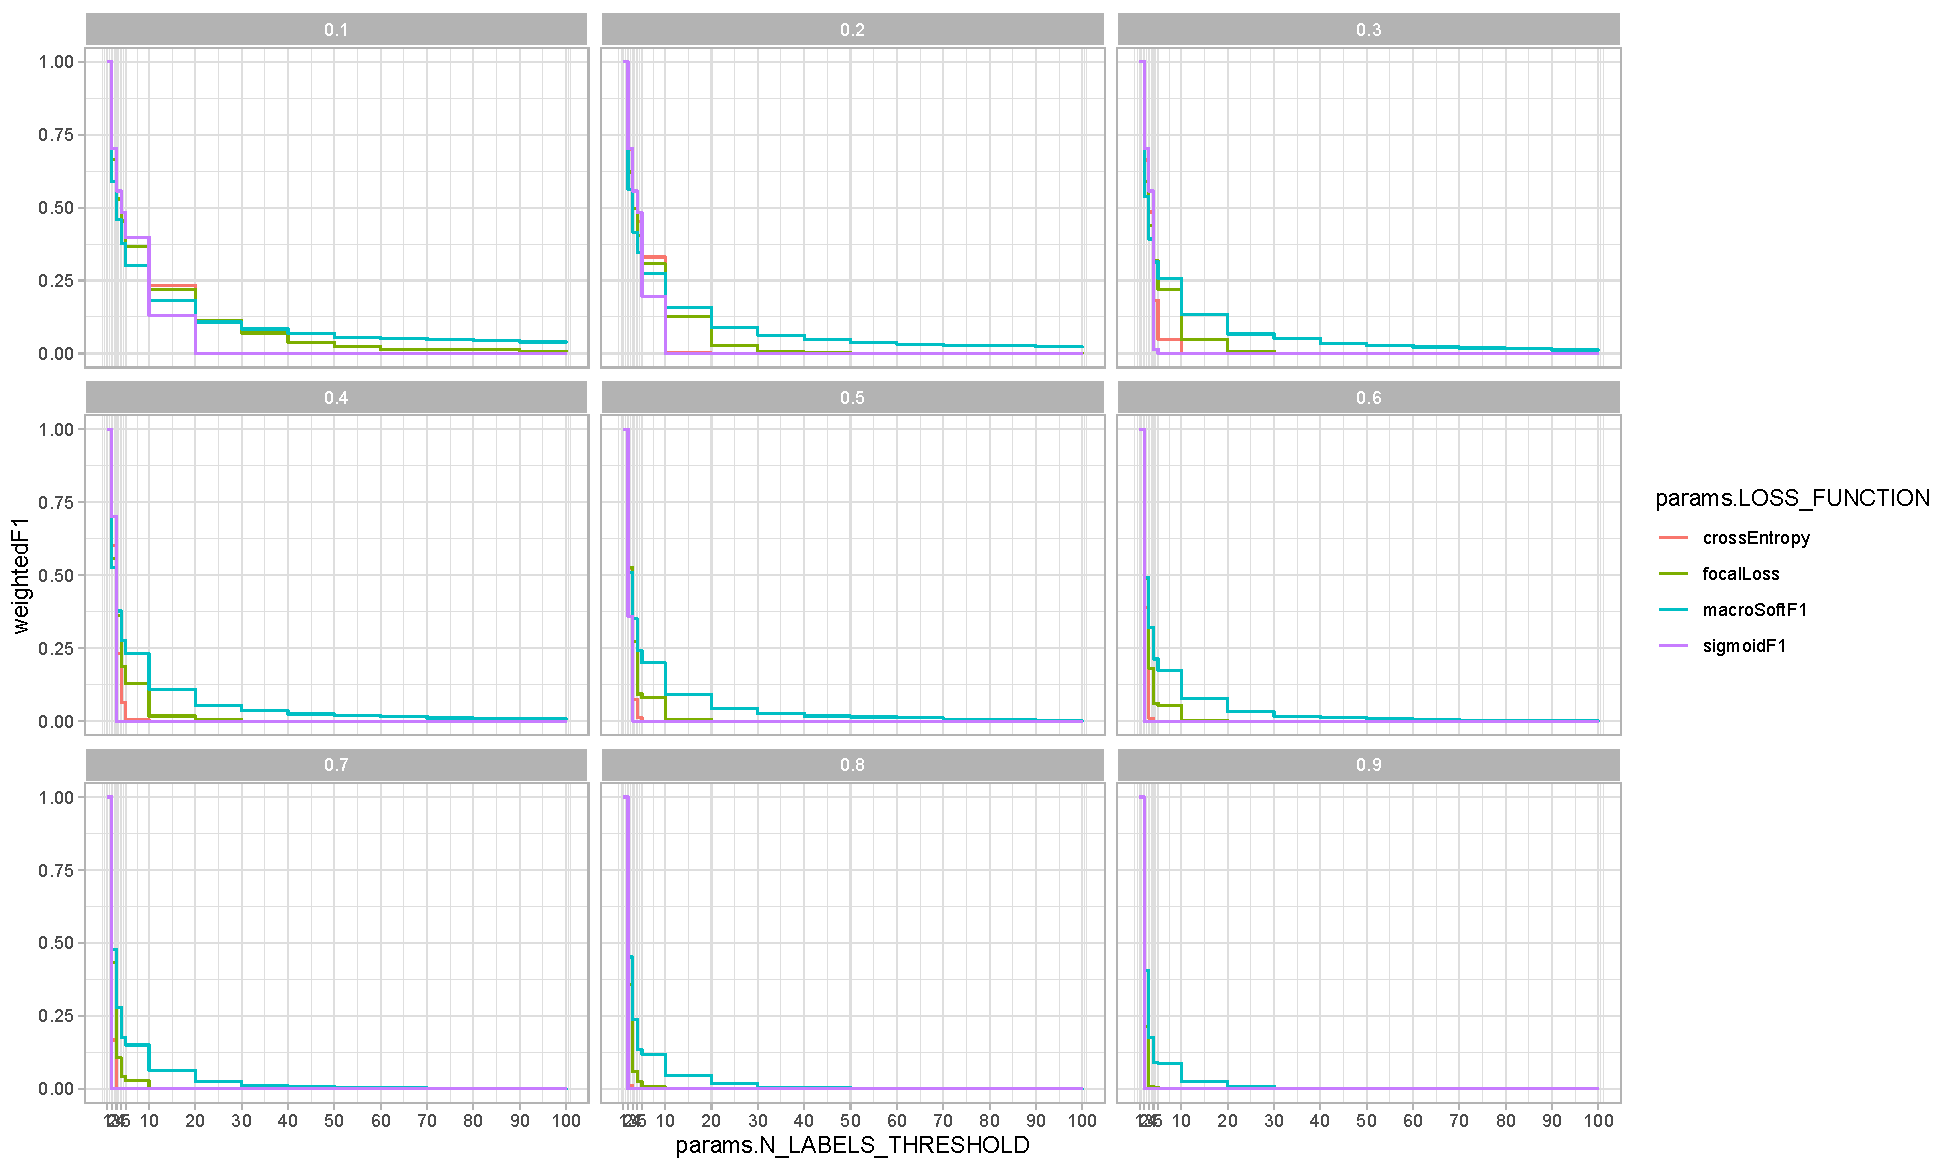
\includegraphics[width=.9\linewidth]{./images/ablation.pdf}
\caption{\label{fig:ablation}
Sigmoid function with different values for $\beta$ (steepness) \& $\eta$ (offset)}
\end{figure}




%%% Local Variables:
%%% mode: latex
%%% TeX-master: "../main"
%%% End:

% !TEX root = ../main.tex

\section{Related Work}
\label{sec:org2aceb9f}

% Beyond identifying object types (see YOLO~\cite{YOLO} and its successors),
% performing face recognition (see FaceNet\cite{FaceNet} and its successors) on
% segments of an image, n
% Neural networks are increasingly becoming better at predicting more abstract
% concepts via deeper networks, representation learning and
% self-supervision~\citep[see, e.g.,][]{SS,Rep}. There is a significant volume
% of recent work on building neural networks with a high-level of abstract
% understanding in the embedding space~\mdr{REF}. However, research on
% developing optimization frameworks that are adapted for these abstract
% concepts in the output space is limited. In the next sections we detail
% some of this related work and discuss it relation to the research in this paper.

Existing algorithmic solutions to deal with FIMPUL tasks can be divided into \emph{fit-data-to-algorithm} solutions, which map FIMPUL problems to a known problem formulation like multiclass uni-label classification, and \emph{fit-algorithm-to-data} solutions, which adapt existing classification
algorithms to the problem at hand~\citep{multilabelMethods}.

\subsection{Fit-data-to-algorithm}
Commonly, in fit-data-to-algorithm solutions, cross-entropy losses are used at training time and thresholding is done at inference time to determine how many labels should be assigned to an instance.
The \textit{label powerset} approach considers each unique set of labels as one class in the transformed setting~\cite{multilabelComparison}.
% (e.g., an instance labeled \textit{Thriller} and \textit{Action}, results in the creation of the class \textit{Thriller and action}).
Alternatively, \textit{ranking by pairwise comparison} is a solution where the dataset is duplicated for each possible label pairs. Each duplicated dataset has therefore two classes and only contains instances that have at least one of the labels in the label pair. Different ranking methods exist~\cite{pairwiseBinary, pairwiseNet}.

More recently, hierarchical datasets such as DBpedia~\citep{lehmann2015dbpedia} are used to finetune BERT-based models~\cite{XLNet, bigBird};  the latter publications use cross-entropy to predict the labels.

\subsection{Fit-algorithm-to-data}
In the fit-algorithm-to-data solutions, elements of the learning
algorithm are changed (such as the back propagation procedure or the task).
Early representatives of fit-algorithm-to-data stem from heterogenous domains
of machine learning. MultiLabel k-Nearest Neighbors \cite{ML-KNN},
MultiLabel Decision Tree \cite{ML-DT}, Ranking Support Vector Machine
\cite{multilabelSVM} and Backpropagation for MultiLabel Learning
\cite{multilabelBackprop}. More recently, two papers introduced the idea of
multi-task learning for \emph{label prediction} and \emph{label count
prediction} for text data \cite[ML\(_{\text{NET}}\)][]{multitaskLabel} and image
data \cite{multitaskLabelImages, tencent}. The latter research is loosely
catered towards object detection and is thus out-of-scope: local elements in a picture are predicted that tend to be uni-label as defined by the ground-truth (e.g., cat, flower, vase, person, bottle
etc.).

An important limitation shared by both \emph{fit-data-to-algorithm} and \emph{fit-algorithm-to-data} is the lack of a holistic approach for both label count and label prediction.

\begin{figure*}[t!]
\centering
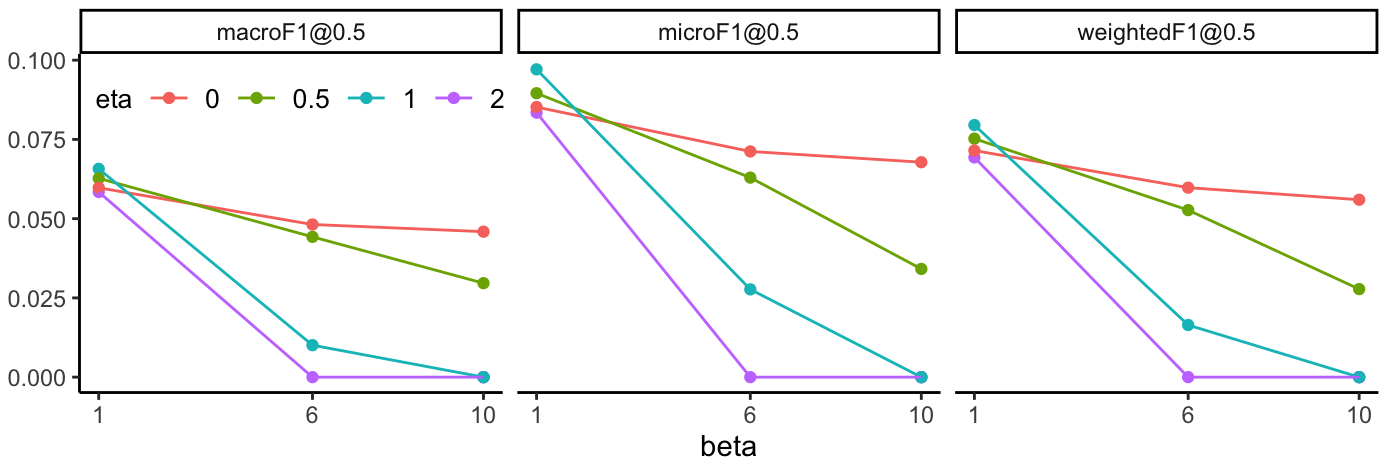
\includegraphics[width=.8\linewidth]{./images/betaEtaResized.png}
\vspace{.5\baselineskip}
\caption{\label{fig:betaEta}
DistilBert (NLP) + classification head on arXiv2020 – different scores at a 0.5 threshold for different values of $\eta$ and $\beta$ in a sampling region similar to Figure~\ref{fig:sigmoid}}
\end{figure*}

\subsection{Thresholding}
\label{subsec:thresh}

Machine learning prediction tasks' output are probabilistic (or a reversible transformation of a probabilistic measure such as a sigmoid or a softmax function).
At training time, these outputs are compared to binary
values in the case of binary encoding of classes.
At inference time, if the number $n_i$ of labels to be predicted per example is known a priori, it is natural to assign the $top_{n_i}$ predictions to that example~\cite{lossTopKError, topKmulticlassSVM}.
If the number of labels per example is unknown a priori,  at inference time the question remains as to how to extract information about the number of labels to assign to each example, aside from the propensity of labels to be assigned.
This is generally done via a \emph{decision threshold}, that can be set globally for all examples, and be
optimized for specificity or sensitivity~\cite{decisionThreshold}.

Thresholding across classes or examples can be an issue when the number of labels to predict is unknown. Some variants of cross-entropy loss accommodate imbalanced label data~\cite{focalLoss}, but remain agnostic to the number of labels to predict.
Solutions include determining an ideal global \emph{threshold} depending on the use-case at hand~\cite{threshForF1}, or per-class-thresholding after training~\cite{moviePosters} and eventually abstracting the threshold away via a \emph{soft-F1} measure~\cite{softF1}.
%In the latter two cases, the task is to predict genre from movie posters.

In our method, this threshold is defined implicitly, thanks to the use of metrics that already penalize for
wrong label counts.


\subsection{Metrics as Losses}

In a number of learning to rank tasks~\cite{LTR}, a model's out of sample accuracy is measured on metrics such as AUROC, F1 score, etc. These reflect an objective catered towards evaluating the model over an entire ranking. Due to the lack of differentiability, these metrics cannot be directly used as loss
functions at training time (in-sample). \citet{optimizableLosses} propose a general framework for deriving
decomposable surrogates from some of these metrics.
Recently, a similar work has been proposed to train a Convolutional
Neural Network (CNN) from scratch with a few millions of images and hundreds
of labels specifically for multilabel tasks \cite{tencent}; this task is loosely related to object detection, similar to \cite{multitaskLabelImages}.
In our research, we instead propose decomposable surrogates of the classical confusion matrix metrics and in particular \emph{sigmoidF1}, tailored to the problem at hand.

% The proposed method is positioned in the lineage of \emph{algorithm
% adaptation}, using \emph{metric as losses} and allowing for dynamic
% \emph{thresholding}.

% This section will be guided by the previous section's formulation of the multitags problem, we will therefore focus on \emph{fit-algorithm-to-data}, \emph{metrics as losses} and \emph{thresholding}.

% \subsection{fit-algorithm-to-data}
% \label{sec:org150a474}

% % Early representatives of \emph{fit-algorithm-to-data} stem from heterogenous domains of machine learning. Multi-Label k-Nearest Neighbors \cite{ML-KNN}, Multi-Label Decision Tree \cite{ML-DT}, Ranking Support Vector Machine \cite{multilabelSVM} and Backpropagation for Multi-Label Learning \cite{multilabelBackprop}. More recently, two papers introduced the idea of multitask learning for \emph{label prediction} and \emph{label count prediction} for text (ML\(_{\text{NET}}\)) \cite{multitaskLabel} and image \cite{multitaskLabelImages} data. The latter research is loosely catered towards object detection (although not formally presented as such) and is thus out-of-scope: elements in a picture are predicted that tend to be unilabel as defined by the groundtruth (e.g. cat, flower, vase, person, bottle etc.).

% \subsection{Metrics as losses}
% \label{sec:orgb0a9d21}

% Often, machine learning post-training evaluation metrics (e.g. AUROC, F1) are not differentiable. There are motivations \todo{which motivations} for optimizing a model directly on a metric at training time. A general framework for AUC, AUROC and F1 is presented in \cite{optimizableLosses}, but the proposed F1 surrogate remains short of being explicitly derived for stochastic gradient descent. \todo{check again with the authors if I can't get inspired from their work}. Recently, a similar work has been proposed to train a Convolutional Neural Network (CNN) from scratch with a few millions of images and hundreds of labels specifically for multilabel tasks \cite{tencent}. This task is loosely related to object detection, similarly to \cite{multitaskLabelImages} mentioned in the previous paragraph.


% in reformulating loss functions to accomodate sparsity in the data, to optimize directly for the metric at hand or to do thresholding posthoc (see movie posters).

% \subsection{Thresholding}
% \label{sec:org8295f09}

% \emph{thresholding} accross classes or examples can be an issue as soon as the number of labels to predict is unknown. Certain variants of cross-entropy loss accommodate imbalanced label data  \cite{focalLoss}, but remain agnostic towards the number of labels to predict. Solutions have been tailored to that end, starting with determining an ideal global \emph{threshold} depending on use-cases \cite{threshForF1}, or per-class-thresholding after training \cite{moviePosters} and eventually abstracting the threshold away via a \emph{soft-F1} measure \cite{softF1} \todo{say more about this method}. In the latter two cases, the task is to predict genre from movie posters.



% The proposed method is positioned in the lineage of \emph{fit-algorithm-to-data}, using \emph{metric as losses} and allowing for dynamic \emph{thresholding}.

% \todo{compare to this:} \cite{lossComp}

% \todo{Hamming Loss}
% % \todo{Precision@K, Recall@K, NDCG@K}
% \todo{MLTSVM loss and the three-way loss inspired by it} \cite{MLTSVM} and \cite{MLTSVMThreeway}

% We propose a dynamic thresholding mechanism auto-tuned at training time.


% ** weak labels
% (unsure the labels are correct)

% - https://people.cs.pitt.edu/~kovashka/ye_zhang_kovashka_iccv2019_cap2det.pdf


% ** implementations

% *** movies

%  [[https://www.analyticsvidhya.com/blog/2019/04/build-first-multi-label-image-classification-model-python/][movie posters with classes]].

%  They have movie titles in them

% *** pretrained resnet on multilabel

%  https://github.com/Tencent/tencent-ml-images

% What happens when using a Resnet pretrained on multilabels

% *** soft F1 score loss

%  https://github.com/ashrefm/multi-label-soft-f1

% https://www.analyticsvidhya.com/blog/2019/04/build-first-multi-label-image-classification-model-python/



% /Optimizing directly for macro F1: By introducing the macro soft-F1 loss, we could train the model to directly increase the metric we care about: the macro F1-score @ threshold 0.5. We could clearly observe the alignment during training and evaluation on successive epochs. When using this loss, we do not have to tune the decision threshold any more. Imagine a multi-label classification system with hundreds of labels, how unstable the system will be if we have to continuously update the optimal threshold for each label. The macro soft-F1 loss comes to the rescue. By using it, we can keep all thresholds fixed at 0.5 and still get an optimal performance from the training process./



%%% Local Variables:
%%% mode: latex
%%% TeX-master: "../main"
%%% End:

% !TEX root = ../main.tex

\section{Conclusion}
\label{sec:orged3d8a1}
% \mdr{Structure the conclusion in five paragraphs, devoted to the following questions:}
% \begin{itemize}[leftmargin=*]
% \item What did we do
% \item What did we find
% \item What are the implications
% \item What are the limitations
% \item What should we do next
% \end{itemize}


\paragraph{Results}
In this paper, we defined a new problem that we call Full-Instance, Multilabel Prediction for Unknown Label count (FIMPUL). It is a subdomain of multiclass classification where an instance needs to be considered as a whole (movie, paper abstract) in order to be labeled. The available labels are from different classes and can be of different numbers per example. This problem is getting addressed more frequently with advances in deep learning providing abstract representation of the input space for multiple modalities that can be used to effectively solve downstream tasks (e.g. with models of the BERT and CNN families). 

To address FIMPUL problems, we proposed a general loss framework for confusion metrics metrics (CoMMaL). We performed  experiments with a specific loss function from the CoMMaL framework, sigmoidF1. We found that sigmoidF1 can achieve significantly better results for most metrics on four diverse datasets and that sigmoidF1 outperforms other losses on the weightedF1 metric.

More generally, CoMMaL, our smooth formulation of confusion matrix metrics allows to optimize directly for these metrics that are usually reserved for the evaluation phase. 

\paragraph{Limitations}
We evaluate the CoMMaL framework and sigmoidF1 loss function only on FIMPUL problems. It can be worth to consider the effectiveness of the CoMMaL framework in different domains. More experimentation is also needed to find a proper heuristic for finetuning sigmoidF1's hyperparameters. However, we do point out that the proposed unboundedF1 counterpart does not require tuning and delivered better results than existing multiclass losses on most metrics. It can act as a less mathematically robust substitute of sigmoidF1.

% It is also debatable whether that niche is 
% it is debatable wether any task is intrinsincly multilabel and wether the image / text cannot be decomposed in parts that are single labeled.

% % not long training and small models, but aibility to demonstrate the statement anyways.



\paragraph{Future work}
In future work, we would like to test the limits of CoMMaL and sigmoidF1 both within and beyond the FIMPUL setting.

But first, if provided enough computing power, one could perform the same experiments with micro losses: given enough representatives of each confusion matrix quadrant for each class, one could consider formulating a micro F1 as a loss. The case where the number of classes is small, the dataset is sizeable and enough memory is available (especially with the recent advances in model parallelism) would be favorable to that end.

%% future work %%
% datasets
% labeling setting
% neural architecture
% SOTA transfer learning
% train from scratch

A first step within the FIMPUL setting, could be to use more robust transfer learning / finetuning procedures, for example with dynamic weight freezing for finetuning~\cite{ULMFit}. Alternatively, we would like to implement the smooth losses to train a CNN or a BERT model for FIMPUL tasks from scratch (c.f., \cite{tencent} and \cite{focalLoss}). If training from scratch, it might then be interesting to combine the proposed loss functions with representation learning \cite{unsupervisedImage,highResRepresentation} or self-supervised learning, in order to model abstract relationships between the labels.

Furthermore, we propose to tackle other multilabel settings, such as hierarchical multilabel classification \cite{HARAM},  active learning (for both see \cite{activeLearningMultiLabel}) or \emph{extreme} multilabel prediction \cite{extremeMultilabelText, extremeSIGIR}, where the number of classes range in the tens of thousands. More generally, sigmoidF1 could be tested on any model that use F1 score as an evaluation metric such as AC-SUM-GAN \cite{AC-SUM-GAN}.

The recently emerged \textit{holistic} content labeling tasks might be another promising testing ground for CoMMaL and sigmoidF1. Holistic labeling refers to labels given to an entire content (full-instance) at different levels of abstraction. A dataset was recently released for \emph{Large Scale Holistic Video Understanding} \cite{holisticVideoData}\footnote{Available at https://github.com/holistic-video-understanding/HVU-Dataset}.

\vspace{\baselineskip}

In the mean time, if this paper is accepted, we will release our results on Kaggle website for the Arxiv multi-label text classification task\footnote{https://www.kaggle.com/Cornell-University/arxiv/tasks?taskId=1757} in the months to come.




%%% Local Variables:
%%% mode: latex
%%% TeX-master: "../main"
%%% End:


\section*{Reproducibility}
To facilitate the reproducibility of the reported results, this work only made use of publicly available datasets and our experimental implementation is publicly available at [URL withheld for double blind review].

\begin{acks}
 This work was supported by many people.
 All content represents the opinion of the authors, which is not necessarily shared or endorsed by their respective employers and/or sponsors.
\end{acks}

\bibliographystyle{ACM-Reference-Format}
\bibliography{references}

\end{document}


%%% Local Variables:
%%% mode: latex
%%% TeX-master: t
%%% End:
